\documentclass[lineno]{jfm}

\usepackage{showframe}
\usepackage{subcaption}
\usepackage{acro}

%%%%%%%%%% additional definitions %%%%%%%%%%
\newcommand\dstar{{\delta^*}} % displacement thickness
\DeclareMathOperator{\argmax}{arg\,max}

% acronyms
\DeclareAcronym{BFS}{short=BFS, long=backward-facing step}
\DeclareAcronym{FFS}{short=FFS, long=forward-facing step}
\DeclareAcronym{LSA}{short=LSA, long=linear stability analysis}
\DeclareAcronym{DNS}{short=DNS, long=direct numerical simulation}
\DeclareAcronym{TS}{short=TS, long=Tollmien--Schlichting}
%%%%%%%%%%%%%%%%%%%%%%%%%%%%%%%%%%%%%%%%%%%%

\lefttitle{V. Ballester Ribó, J. D. Crouch, Y. Hwang and S. J. Sherwin}
\righttitle{Journal of Fluid Mechanics}

\title{Transition over surface gaps in incompressible laminar boundary layers}

\author{Víctor Ballester Ribó\aff{1}, Jeffrey D. Crouch\aff{2}, Yongyun Hwang\aff{1} \and Spencer J. Sherwin\aff{1}}

\affiliation{\aff{1}Department of Aeronautics, Imperial College London, South Kensington, London SW7 2AZ, UK
\aff{2}The Boeing Company, P.O. Box 3707, Seattle, WA 98124-2207, USA}

\corresau{Víctor Ballester Ribó, \email{v.ballester-ribo24@imperial.ac.uk}}

\begin{document}
% lineno-FLM.sty (loaded by jfm.cls at \begin{document}) re-issues
% \newif\ifLineNumbers *after* \runninglinenumbers, which resets lineno's own
% flag to false and silently disables \linenomath.  The consequence is that the
% part of a paragraph preceding a display equation gets no line numbers.
\LineNumberstrue
\maketitle

\begin{abstract}
	Experiments have shown that sufficiently large surface gaps at aircraft panel joints cause transition to jump onto the gap itself, but the mechanism behind this bypass transition is not fully understood. Here, the effect of a spanwise-uniform rectangular gap on the stability and transition of incompressible laminar boundary layers is investigated by \acl{DNS} and \acl{LSA}, for gap widths $w\in[0,130]$, depths $d\in[0,4]$ and Reynolds numbers $\Rey_\dstar\in[800,3000]$, all based on the displacement thickness $\dstar$ at the gap. Narrow or shallow gaps leave the flow steady. The gap then acts solely as an amplifier of incoming \acl{TS} waves, adding an increment $\Delta n$ to their smooth-wall amplification factor $n$. Transition remains downstream of the gap, although upstream of the smooth-wall location. Wider or deeper gaps destabilise the steady flow, and the depth determines whether the first instability is two-dimensional (spanwise-uniform) or three-dimensional (spanwise-varying). Shallow gaps first become unstable to two-dimensional perturbations, and the flow settles onto a limit cycle, a self-sustained oscillation of the gap. Deep gaps first become unstable to three-dimensional perturbations, which saturate without breakdown. Transition moves onto the gap precisely where the two-dimensional limit cycle is itself unstable to three-dimensional perturbations, a criterion that reproduces the bypass transition boundary measured experimentally. The analysis shows that the two- and three-dimensional instabilities are together necessary and sufficient for transition to occur at the gap.
\end{abstract}

% acronyms used in the abstract should not count as first use
\acresetall

\section{Introduction}\label{sec:introduction}
Aircraft surfaces which are designed to sustain laminar flow must also conform to manufacturing requirements. Panel joints, access doors and control-surface seams leave steps and gaps whose dimensions are then set by manufacturing tolerances. Near a transport-aircraft nacelle's leading edge the displacement thickness is only $\dstar\sim O(0.1\,\mathrm{mm})$, so a millimetre gap spans several $\dstar$ and can move transition far upstream. However, tolerances are expensive to tighten, and therefore the question is not whether gaps can be removed but how large one may be before it matters.

Under the quiet free stream of flight, a boundary layer follows the classical route to turbulence: \ac{TS} waves are excited by receptivity, amplify convectively and break down at finite amplitude. In practice this sequence is reduced to the $e^{n}$ method \citep{smithgamberoni,vanIngen1956}, which integrates the amplification factor $n(x)$ and declares transition where it reaches a threshold $N$ calibrated to the disturbance environment \citep{crouchNgKachanov2015}. Extending the method to an imperfect surface can be done in two ways.  Either it increases the amplification, by the increment $\Delta n=n_\mathrm{gap}(x)-n_\mathrm{flat}(x)$, over the smooth-wall curve at fixed $N$, or it lowers the threshold, by the drop $\Delta N$ in $n_\mathrm{flat}$, between the transition locations measured without the imperfection and with it \citep{crouchKosoryginNg2006,perraudArnalKuehn2014,crouch2021predicting}. However, both methods rely on the same premise: the imperfection amplifies waves reaching it from upstream and creates none of its own.

This premise, however, holds only up to a certain gap size. Early design criteria for laminar-flow-control surfaces already limited the gap width through a gap-width Reynolds number, of about $15\,000$, beyond which transition moves significantly forward \citep{nenniGluyas1966}, without accounting for the gap depth or identifying a mechanism. Laminar cavities were later classified into open and closed regimes, according to whether the separated shear layer reattaches to the cavity floor \citep{sinhaGuptaOberai1982,Zhang2005,Crook2013}, which indicates that a sufficiently large gap changes the flow qualitatively rather than merely perturbing it. ONERA experiments \citep{oliveBlanchard1982,seraudie2010,gentili2012} then varied the gap width $w$ and depth $d$ independently and mapped, in the $(w,d)$ plane, the threshold beyond which transition occurs at the gap itself, that is, where the premise fails. Below this threshold, \citet{beguetONERA} found the depth to have a negligible effect on $\Delta N$ for gaps with aspect ratio $0.2<d/w<0.7$. For deep gaps, $d/w>5$, the compressible simulations of \citet{zahnRist} at $M=0.6$ instead found a non-monotonic dependence of $\Delta n$ on depth, which they attributed to an acoustic feedback whose resonance condition is set by the depth.

Only recently has the $(w,d)$ plane been swept systematically in a single facility. The experiments of \citet{jeffGaps}, at low Mach number ($M<0.1$) and low free-stream turbulence, span $0<w<110$ and $0<d<11$ and show that, wherever \ac{TS} waves still control transition, the data follow one of two limiting regimes selected by the aspect ratio. For $d/w\to 0$ the \ac{BFS} result $\Delta N=4.4d$ applies independently of $w$ while for $d/w\to\infty$, $\Delta N\approx0.1w$ applies independently of $d$. Beyond a boundary lying within $d\gtrsim1.8$ and $w\gtrsim19$, neither of these formulas holds: transition moves onto the gap itself and occurs at a markedly higher frequency, outside the \ac{TS} band. These points were labelled \emph{bypass} transition and excluded from the correlations.

This gap-located transition has been examined most directly by Medeiros and co-workers, all in compressible subsonic flow. Using global stability analysis at Mach numbers in the range $0.1\leq M\leq0.5$, \citet{mathiasMedeiros2019} attributed it to an instability of the shear layer spanning the gap, sustained by the edge-to-edge feedback loop of \citet{rossiter1964}. Extending the range to $0.1\leq M\leq0.9$, \citet{mathiasMedeiros2021} showed that the thickness of the incoming boundary layer selects which Rossiter mode dominates, whereas the Mach number controls the acoustic energy transfer that closes the feedback loop. Thus, compressibility was found to be strongly destabilising even at low $M$. Finally, at $M=0.5$, \citet{aguirreMedeiros2024} partitioned the $(w,d)$ plane into three regions: one in which all modes are stable, one in which only three-dimensional (spanwise-periodic) centrifugal modes are unstable, and one in which two-dimensional (spanwise-uniform) Rossiter modes are unstable as well. The boundary of this last region lies close to the bypass boundary of \citet{jeffGaps}. However, the nonlinear evolution of the three-dimensional modes, and how they interact with the two-dimensional ones, has received little attention.

Two questions are therefore left open. The first concerns gaps that act as amplifiers: what mechanism sets the increment $\Delta n$, and why gaps of different width and depth amplify differently. The second concerns the bypass transition itself: what sets the boundary beyond which transition moves onto the gap. The amplifier description underlying both $\Delta n$ and $\Delta N$ fails once the gap sustains an instability of its own, but linear instability marks only where the steady flow ceases to exist, not where transition occurs, since a saturated unstable mode may or may not break down. Answering the second question therefore requires following the unstable modes beyond saturation, to establish at what stage the flow becomes three-dimensional and whether the two- and three-dimensional instabilities act independently, compete or reinforce one another. This interaction has no counterpart in the canonical cavity literature \citep{GharibRoshko1987,dynandcontrol,bresColonius2008,Citro2015}, in which the cavity sits in an otherwise stable stream rather than in a boundary layer that is itself convectively unstable.

We address these questions using \ac{DNS} and global and local stability analysis \citep{huerreMonkewitz1990,chomaz2005,theofilis2011} of incompressible flow over a spanwise-uniform rectangular gap, for $w\in[0,130]$, $d\in[0,4]$ and $\Rey\in[800,3000]$, where $w$ and $d$ are nondimensionalised by the displacement thickness $\dstar$ at the gap and $\Rey=u_\infty\dstar/\nu$, with $u_\infty$ the free-stream velocity. This range of Reynolds numbers is representative of the leading-edge region of a transport-aircraft nacelle at cruise conditions. The whole range lies entirely above the critical Reynolds number $\Rey_\mathrm{c}\approx520$ beyond which the Blasius boundary layer becomes convectively unstable. Within this range, $\Rey=1000$ is taken as the reference condition because it is the Reynolds number at which \citet{jeffGaps} measured both $\Delta N$ and the bypass transition boundary, against which the present results are compared. The picture that emerges at $\Rey=1000$ is summarised in figure~\ref{fig:introMap}. 

\begin{figure}[ht]
	\centering
	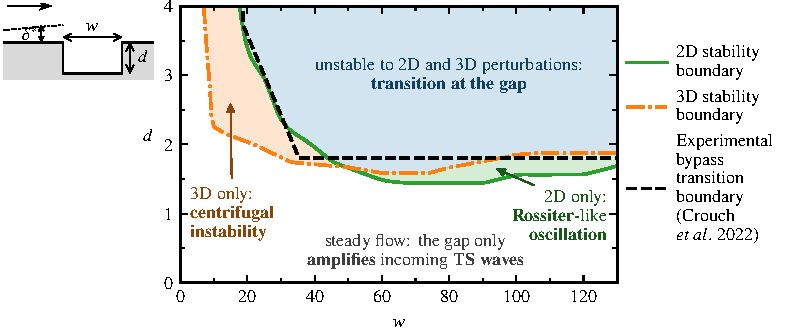
\includegraphics{Images/introRegimeMap.pdf}
	\caption{Overview of the results at $\Rey=1000$, in the plane of gap width $w$ and depth $d$ nondimensionalised by $\dstar$. Below both stability boundaries the flow over the gap is steady and the gap only amplifies \ac{TS} waves arriving from upstream. Crossing a single boundary gives either a saturated three-dimensional state (orange) or a self-sustained two-dimensional oscillation (green), neither of which breaks down on its own at the gap, although the disturbances they release into the boundary layer advance transition downstream of the gap. Transition moves onto the gap only once both boundaries are crossed (blue), and the upper envelope of the two boundaries follows the bypass transition boundary measured by \citet{jeffGaps} (dashed). The boundaries are computed in Section~\ref{sec:globalStability}.}\label{fig:introMap}
\end{figure}
Narrow and shallow gaps settle onto an equilibrium and act purely as amplifiers, raising the amplification factor of incoming \ac{TS} waves above its smooth-wall value by an increment $\Delta n$. Local analysis shows that $\Delta n$ is set by a competition between two factors: the range of frequencies destabilised by the cavity shear layer, and the streamwise distance over which this destabilisation acts. Wider or deeper gaps destabilise the equilibrium, and the depth determines whether the first instability is two- or three-dimensional: shallow gaps lose stability to two-dimensional perturbations first and settle onto a limit cycle, whereas deep gaps lose stability to three-dimensional perturbations, which saturate without breaking down. Transition occurs at the gap precisely where the two-dimensional limit cycle is itself unstable to spanwise-varying perturbations, a criterion that reproduces the measured bypass boundary. Both instabilities are therefore necessary, and the onset of transition at the gap is set by a bifurcation of the flow thus explaining the empirically-determined threshold.

The paper is organised as follows. Section~\ref{sec:numericalSetup} presents the governing equations and the numerical methods employed to solve them. Section~\ref{sec:globalStability} computes the equilibrium base flows and their linear stability to spanwise-uniform and spanwise-varying perturbations. Section~\ref{sec:2Ddynamics} examines the two-dimensional dynamics: the amplification increment $\Delta n$ where the equilibrium is stable, and the limit cycles that emerge once the equilibrium loses stability. Section~\ref{sec:3Ddynamics} follows the nonlinear three-dimensional dynamics and tests the limit cycles for stability to spanwise-varying perturbations, which yields the transition scenarios at the gap. Section~\ref{sec:conclusions} summarises the results.

\section{Numerical setup}\label{sec:numericalSetup}
The incompressible Navier--Stokes equations are solved using a spectral/\textit{hp}-element formulation. In nondimensional form, the governing equations are
\begin{equation}\label{eq:ns}
	\begin{aligned}
		\partial_t \boldsymbol{u} + (\boldsymbol{u}\cdot\bnabla)\,\boldsymbol{u} & = -\bnabla p + \frac{1}{\Rey} \nabla^2 \boldsymbol{u}, \\
		\bnabla \cdot \boldsymbol{u}                                       & = 0,
	\end{aligned}
\end{equation}
where $\boldsymbol{u}={(u_x,u_y,u_z)}^\mathrm{T}$ denotes the velocity field, $p$ is the pressure, and $\Rey$ is the Reynolds number. Throughout the paper, $\boldsymbol{x}={(x,y,z)}^\mathrm{T}$ denotes the Cartesian coordinates, with $x$, $y$ and $z$ denoting the streamwise, wall-normal and spanwise directions, respectively. In \eqref{eq:ns}, $\boldsymbol{u}\cdot\bnabla:=u_x\partial_x+u_y\partial_y+u_z\partial_z$, $\bnabla\cdot{}$ denotes the divergence operator and $\nabla^2$ denotes the Laplacian. The scalar operators $\boldsymbol{u}\cdot\bnabla$ and $\nabla^2$ act on each component of a vector. The equations are nondimensionalised using the streamwise component of the free-stream velocity, $u_\infty$, as the characteristic velocity and the displacement thickness $\dstar$ as the characteristic length scale. The latter is evaluated at the upstream edge of the gap for the smooth-wall reference flow. Thus,
$
	\Rey \equiv \Rey_\dstar := u_\infty \dstar/\nu
$,
where $\nu$ is the kinematic viscosity of the flow. The Reynolds number is varied in the range $\Rey \in [800,3000]$. All the quantities in the paper are nondimensional unless otherwise stated.

All simulations are performed using the \texttt{Nektar++} solver \citep{nektar}, configured with a velocity-correction scheme and a continuous Galerkin projection \citep{vcs1,vcs2}. Time integration is performed using a second-order IMEX scheme, with the viscous terms treated implicitly and the advection term treated explicitly. Spectral vanishing viscosity is added to stabilise the numerical scheme in regions containing sharp gradients \citep{svv}.

The computational domain $\Omega$ is a rectangular cuboid, with a cavity of width $w$, depth $d$ and spanwise-uniform geometry attached to the lower wall to model the surface gap (figure~\ref{fig:domain}). The origin, $\boldsymbol{x}=\boldsymbol{0}$, is located at the upstream edge of the gap on the outermost spanwise plane. The domain dimensions are $h=150$, $\ell_{\mathrm{i}}=100$ and $\ell_{\mathrm{o}}=1000$, which are chosen to ensure a fully developed upstream boundary layer and to minimise the influence of the upper and downstream boundaries on the region of interest. The spanwise length is set to $b=4d$, which is sufficient to capture the relevant three-dimensional dynamics (see Section~\ref{sec:globalStability}). A spanwise-uniform Blasius profile ($\boldsymbol{u}=\boldsymbol{u}_\mathrm{bla}(y)$) is prescribed at the inlet and no-slip conditions ($\boldsymbol{u}=\boldsymbol{0}$) are imposed on the solid walls. At the upper boundary, a far-field condition ($\boldsymbol{u}=\boldsymbol{u}_\mathrm{far}(x)$) is imposed. At the outlet, the outflow boundary condition of \citet{dong} is used to minimise numerical instabilities when energetic vortices leave the computational domain. Periodic boundary conditions are imposed in the spanwise direction.

\begin{figure}[ht]
	\centering
	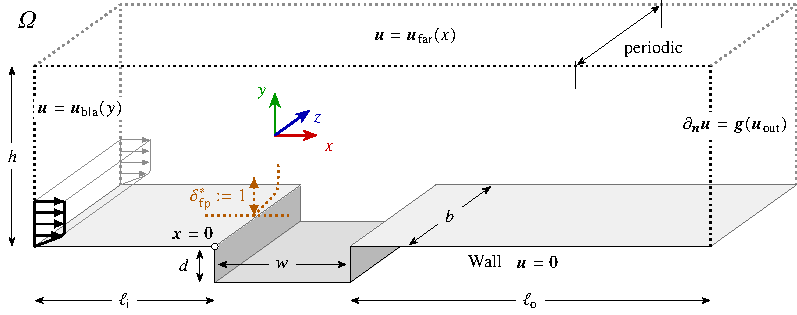
\includegraphics{Images/domainBaseflow3D.pdf}
	\caption{Computational domain used throughout the study. The gap is spanwise uniform, of width $w$ and depth $d$, and the domain is periodic in the spanwise direction with spanwise length $b$. Boundary conditions are shown for the nonlinear simulations, where the function $\boldsymbol{g}$ in the outlet denotes \citet{dong} outflow condition. The orange marker is the displacement thickness $\dstar$ of the smooth-wall reference flow at the upstream edge of the gap, which sets the reference length. The dimensions are anisotropically rescaled for clearer visualisation of the gap geometry.}\label{fig:domain}
\end{figure}
The domain is discretised using a Fourier expansion in the homogeneous spanwise direction, combined with a spectral/\textit{hp} element discretisation in each Fourier plane. Within a plane, a structured mesh of quadrilateral elements is used in the boundary-layer region and unstructured triangular elements in the far field. Between 4000 and 7000 elements are used in each simulation, depending on the gap geometry. On each element, polynomial orders 5 and 4 are used to approximate the velocity and the pressure fields, respectively. This choice satisfies the inf-sup condition and prevents the numerical instabilities associated with an incompatible velocity-pressure discretisation \citep[see][]{infsupCondition,infsupTaylorHood}. The polynomial basis is constructed from modified hierarchical Jacobi polynomials of the corresponding dimensions \citep{spectralhpSpencerBible}. In the spanwise direction the solution is expanded using 48 homogeneous Fourier modes, so that the full three-dimensional discretisation amounts to approximately $4\times10^{6}$ degrees of freedom. The classical 3/2 padding dealiasing rule is incorporated in the Fourier expansion and a spectral/\emph{hp} dealiasing technique \citep{mengaldo} is used in the spectral/\textit{hp} discretisation to prevent aliasing errors in the nonlinear terms. The resulting spatial resolution is sufficient to resolve the relevant flow features, as confirmed by grid-convergence studies.

For global \ac{LSA}, the Navier--Stokes equations~\eqref{eq:ns} are linearised around a base flow $\boldsymbol{Q}={(U_x,U_y,U_z,P)}^\mathrm{T}$, that is, a base velocity field $\boldsymbol{U}={(U_x,U_y,U_z)}^\mathrm{T}$ and a base pressure field $P$ that together solve~\eqref{eq:ns}. The base flows are obtained from nonlinear simulations of~\eqref{eq:ns} and they can be either an equilibrium solution for standard \ac{LSA} or a periodic orbit for Floquet analysis. When the base flow is globally unstable, the selective frequency damping method \citep{akervik2006,sfd} is used to suppress the unstable modes and obtain the corresponding unstable equilibrium solution. When the base flow is a stable periodic orbit, the periodic orbit is extracted through naive time integration. The state $\boldsymbol{q}={(u_x,u_y,u_z,p)}^\mathrm{T}$ is then decomposed as $\boldsymbol{q}=\boldsymbol{Q}+\boldsymbol{q}'$, where $\boldsymbol{q}'={(u_x',u_y',u_z',p')}^\mathrm{T}$ comprises the perturbation velocity field $\boldsymbol{u}'={(u_x',u_y',u_z')}^\mathrm{T}=\boldsymbol{u}-\boldsymbol{U}$ and the perturbation pressure $p'=p-P$. Substituting this decomposition into~\eqref{eq:ns} and retaining only the terms linear in $\boldsymbol{q}'$ gives the linearised equations, written in compact form as% chktex 8
\begin{equation}\label{eq:linearizedNS}
	\begin{aligned}
		\boldsymbol{\mathcal{M}}\partial_t\boldsymbol{q}'      & = \boldsymbol{\mathcal{L}}(\boldsymbol{U})\boldsymbol{q}',                                                                                                                                                   \\
		\qquad\qquad\boldsymbol{\mathcal{M}} = \begin{bmatrix}
			\boldsymbol{I}_3 & \boldsymbol{0} \\ \boldsymbol{0}^\mathrm{T} & 0 \end{bmatrix},\quad & \boldsymbol{\mathcal{L}}(\boldsymbol{U}) = \begin{bmatrix}
			-\mathcal{C}_{\boldsymbol{U}} + \frac{1}{\Rey}\nabla^2 & -\bnabla \\ \bnabla\cdot{} & 0
		                                                                                                                                    \end{bmatrix},
	\end{aligned}
\end{equation}
where $\boldsymbol{I}_3$ is the identity matrix of size 3 and $\mathcal{C}_{\boldsymbol{U}}\boldsymbol{u}':=(\boldsymbol{U}\cdot\bnabla)\,\boldsymbol{u}'+(\boldsymbol{u}'\cdot\bnabla)\,\boldsymbol{U}$ is the advection operator linearised around $\boldsymbol{U}$. For standard global \ac{LSA}, the base flow is constant in time. For Floquet analysis, the base flow depends on time and it is $T$-periodic, $\boldsymbol{U}(t+T)=\boldsymbol{U}(t)$. For this study, in both cases the base flow is independent of the spanwise coordinate, so perturbations separate into spanwise Fourier modes that evolve independently. Combining this with Floquet's theorem, solutions of~\eqref{eq:linearizedNS} are sought in the form
\begin{equation}\label{eq:floquetansatz}
	\boldsymbol{u}'(x,y,z,t)
	= \hat{\boldsymbol{u}}(x,y,t)\,\mathrm{e}^{\mathrm{i}\beta z}\,\mathrm{e}^{\lambda t},
	\qquad
	\hat{\boldsymbol{u}}(x,y,t+T)=\hat{\boldsymbol{u}}(x,y,t),
\end{equation}
where $\beta$ is the spanwise wavenumber and $\lambda$ is the complex Floquet exponent. For a spanwise-periodic domain of length $b$, the admissible wavenumbers are $\{\beta_k = 2\pi k/b : k=0,\ldots,15\}$. Throughout this paper, perturbations with $\beta=0$ are spanwise-uniform and are referred to as two-dimensional, whereas three-dimensional perturbations are those with $\beta\neq0$, which vary along the span. With this convention, the mode $k=0$, although trivially periodic in $z$, is not counted as three-dimensional. When the base flow is steady, $\hat{\boldsymbol{u}}$ is independent of time and~\eqref{eq:floquetansatz} reduces to the classical normal-mode ansatz. In both cases, the eigenvalue problem is solved with a matrix-free time-stepper approach \citep{tuckermanBarkley2000,barkleyBlackburnSherwin2008}. Integrating the linearised equations~\eqref{eq:linearizedNS} over a time interval $\tau$ defines the monodromy operator $\mathcal{A}(\tau)$, which maps an initial perturbation $\boldsymbol{q}'(0)$ onto $\boldsymbol{q}'(\tau)$. The eigenvalues $\mu$ of $\mathcal{A}(\tau)$ are related to the exponents $\lambda$ by $\mu=\mathrm{e}^{\lambda\tau}$, so that the eigenvalues of largest modulus correspond to the largest growth rates $\Re(\lambda)$. These leading eigenvalues and their eigenmodes are computed with an Arnoldi method that requires only repeated actions of $\mathcal{A}(\tau)$, that is, successive linearised simulations.

Local \ac{LSA} complements the global analysis and is used mainly to interpret the amplification of two-dimensional \ac{TS} waves across the gap. In this framework, the base flow is approximated as locally parallel at each streamwise location, $\boldsymbol{U}=(U(y),0)$, and perturbations are sought as normal modes of the form
\begin{equation}\label{eq:localansatz}
	\boldsymbol{u}'(x,y,z,t)
	=
	\hat{\boldsymbol{u}}(y)\,\mathrm{e}^{\mathrm{i}(\alpha x + \beta z - \omega t)},
\end{equation}
where $\alpha =\alpha_\mathrm{r}  + \mathrm{i}\alpha_\mathrm{i} $ is the complex streamwise wavenumber, $\beta $ the spanwise wavenumber and $\omega =\omega_\mathrm{r} +\mathrm{i}\omega_\mathrm{i} $ the complex frequency. Since \ac{TS} waves are two-dimensional, only $\beta=0$ is considered, and substituting~\eqref{eq:localansatz} into the linearised equations gives the Orr--Sommerfeld problem \citep{schmid2001stability}% chktex 8
\begin{equation}\label{eq:OS}
	{\big({\mathrm{D}}^2-{\alpha}^2\big)}^2\hat{u}_y
	-\mathrm{i}\Rey\left[
		(\alpha U-\omega)\big({\mathrm{D}}^2-{\alpha}^2\big)
		-\alpha U''\right]\hat{u}_y=0,
\end{equation}
for the wall-normal velocity component $\hat{u}_y$, where $\mathrm{D}:=\mathrm{d}/\mathrm{d}y$. The problem is subject to $\hat{u}_y(0)=\mathrm{D}\hat{u}_y(0)=0$ and $\hat{u}_y,\mathrm{D}\hat{u}_y\to0$ as $y\to\infty$. Fixing $\Rey$, the pairs $(\alpha,\omega)$ for which~\eqref{eq:OS} admits a non-trivial solution form the zero set of a dispersion function $\mathcal{D}(\alpha,\omega;\Rey)$. The temporal and spatial formulations are two different real restrictions of this same zero set: the temporal one prescribes $\alpha=\alpha_\mathrm{r}\in\mathbb{R}$ and solves for $\omega$, whereas the spatial one prescribes $\omega=\omega_\mathrm{r}\in\mathbb{R}$ and solves for $\alpha$. In this work, only the spatial formulation has been used (see Section~\ref{sec:2Dstable}). Equation~\eqref{eq:OS} is discretised by Chebyshev collocation on $81$ Gauss--Lobatto points, with the domain truncated at $y_{\max}=45$. The points are clustered near the wall by the algebraic mapping of \citet{malik1990}. Following \citet{bridgesMorris1984}, the auxiliary variable $\hat{q}=({\mathrm{D}}^2-\alpha^2)\hat{u}_y$ is introduced to reduce it to a quadratic problem in $\alpha$, which is then linearised into a generalised eigenvalue problem and solved with the QZ algorithm. Each streamwise station and frequency is solved independently, and the \ac{TS} mode is selected from the full spectrum as the least damped eigenvalue whose phase speed lies in $0.15<\omega_\mathrm{r}/\alpha_\mathrm{r}<0.75$.

\section{Global stability analysis}\label{sec:globalStability}
\subsection{Base flows}
For sufficiently small gap depths and widths, the flow asymptotically approaches an equilibrium state (i.e.\ laminar steady base flow), provided that the initial condition lies within its basin of attraction. The equilibrium flow topology in the boundary layer outside the gap remains close to a Blasius profile, while the flow topology inside the cavity changes strongly with the cavity aspect ratio $w/d$ (figure~\ref{fig:baseflow}).

\begin{figure}[ht]
	\begin{subfigure}{0.33\linewidth}
		\centering
		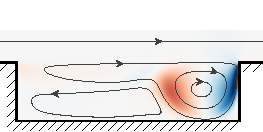
\includegraphics{Images/2dstates/pdfs/gapd4_w15.pdf}
		\caption{$w=15$, $d=4$}\label{fig:baseflowA}
	\end{subfigure}
	\begin{subfigure}{0.33\linewidth}
		\centering
		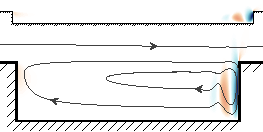
\includegraphics{Images/2dstates/pdfs/gapd1.5_w30.pdf}
		\caption{$w=30$, $d=1.5$}\label{fig:baseflowB}
	\end{subfigure}
	\begin{subfigure}{0.33\linewidth}
		\centering
		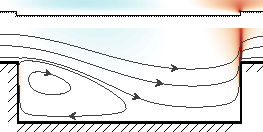
\includegraphics{Images/2dstates/pdfs/gapd1_w60.pdf}
		\caption{$w=60$, $d=1$}\label{fig:baseflowC}
	\end{subfigure}\\[10pt]
	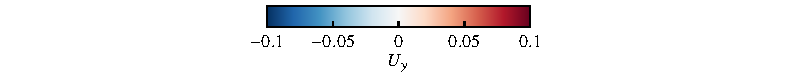
\includegraphics{Images/2dstates/pdfs/colorbar_equilibrium.pdf}
	\caption{Equilibrium solutions (laminar steady base flow) for three representative gap geometries shown using wall-normal-velocity contours ($U_y$) and streamlines. All geometries are rescaled to match the aspect ratio of the first case ($w/d = 15/4$) for visual comparison; the original unscaled domain profiles are shown above the last two panels.}\label{fig:baseflow}
\end{figure}
For small $w/d$ (figure~\ref{fig:baseflowA}), a recirculation vortex forms within the cavity beneath the shear layer spanning the gap. This topology is characteristic of an open cavity, for which the separated shear layer remains detached from the cavity floor and the cavity interior is dominated by recirculating flow \citep{sinhaGuptaOberai1982,Crook2013}.

Increasing the aspect ratio $w/d$ (figure~\ref{fig:baseflowB}) produces a more elongated, shallow recirculation region. The internal reverse flow is increasingly confined in the wall-normal direction, while the flow still features a recirculation vortex in the vicinity of the downstream edge of the gap.

Increasing $w/d$ further (figure~\ref{fig:baseflowC}), the cavity is very shallow and the recirculating motion is confined predominantly to a region adjacent to the upstream edge of the gap. In contrast to the deep-cavity case, the outer shear layer exhibits strong streamwise curvature. The resulting structure approaches the closed-cavity topology, for which the separated shear layer reattaches to the cavity floor before leaving the cavity \citep{Zhang2005}.

In the limit $w/d\to\infty$, the two cavity steps become asymptotically separated in the streamwise direction, and the flow may be interpreted locally as a \ac{BFS} flow in the vicinity of the upstream edge and a \ac{FFS} flow near the downstream edge. The shear layer separated from the upstream step extends across the gap and becomes increasingly less affected by the downstream edge. The associated recirculation remains confined near the upstream step. Near the downstream edge, the shear layer hits the wall and is deflected back into the external flow, resulting in a flow topology similar to that of \iac{FFS}.

\subsection{Stability of the base flows}
To assess the stability of the equilibrium states, a biglobal stability analysis is performed for both two-dimensional (spanwise-uniform, $\beta=0$) and three-dimensional (spanwise-varying, $\beta\neq0$) perturbations. The stability of base flows with respect to two-dimensional disturbances is characterised by the growth rate
\begin{equation}
	\sigma_{\mathrm{2D}}(w,d)
	=
	\max
	\big\{
	\Re(\lambda):
	\lambda\in
	\mathrm{spec}\big(
	\mathcal{L}_{w,d}^{\beta_0}
	\big)
	\big\},
\end{equation}
where $\mathcal{L}_{w,d}^{\beta_k}$ denotes the discretised linearised operator of~\eqref{eq:linearizedNS} for the gap configuration $(w,d)$ and spanwise wavenumber $\beta_k$, and $\mathrm{spec}(\cdot)$ denotes the spectrum of the operator. For three-dimensional perturbations, the leading eigenvalue is computed for the range of spanwise wavenumbers $\beta_k$ described above, and the maximum growth rate over these wavenumbers is retained,
\begin{equation}\label{eq:sigma3D}
	\sigma_{\mathrm{3D}}(w,d)
	=
	\max_{k=1,\ldots,15}
	\max
	\big\{
	\Re(\lambda):
	\lambda\in
	\mathrm{spec}\big(
		\mathcal{L}_{w,d}^{\beta_k}
	\big)
	\big\}.
\end{equation}
For every gap considered and $\Rey=1000$, the maximum in~\eqref{eq:sigma3D} is attained around $\beta_9$ or $\beta_{10}$, well inside the sampled range, and the growth rate at the largest wavenumber $\beta_{15}$ is small compared with this maximum. The set $\{\beta_k\}_{k=0}^{15}$ therefore contains the most unstable wavenumber and is sufficient to capture the leading three-dimensional instability.

The onset of instability is determined by identifying the values of $w$ and $d$ for which $\sigma_{\mathrm{2D}}$ and $\sigma_{\mathrm{3D}}$ become positive. This procedure defines the two-dimensional and three-dimensional stability boundaries in the $(w,d)$ plane. The subscripts 2D and 3D are used throughout to label quantities associated with two-dimensional and three-dimensional perturbations, respectively. The frequency of the most unstable two-dimensional mode is given by
\begin{equation}
	\omega_{\mathrm{2D}}
	=
	\Im\left(\argmax\big\{\Re(\lambda) : \lambda \in\mathrm{spec}(\mathcal{L}_{w,d}^{\beta_0})\big\}\right),
\end{equation}
and analogously for the frequency $\omega_\mathrm{3D}$ of the three-dimensional modes. Figure~\ref{fig:3d2dDynamics1000} compares the resulting stability boundaries with the experimental bypass transition boundary reported by \citet{jeffGaps} at $\Rey=1000$.

\begin{figure}[ht]
	\centering
	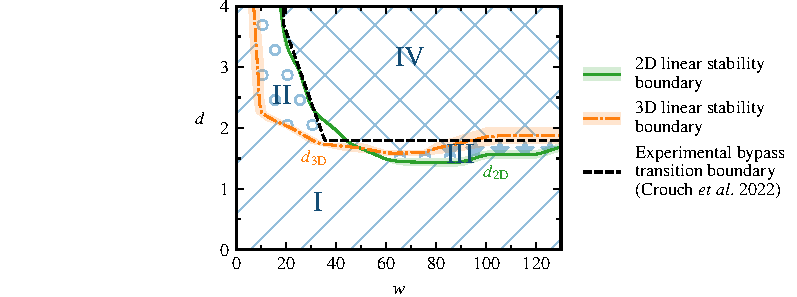
\includegraphics{Images/3d2dStabilityCurveRe1000.pdf}
	\caption{Two-dimensional (solid green line) and three-dimensional (dash-dotted orange line) linear stability boundaries in the $(w,d)$ plane at $\Rey=1000$. Shaded bands indicate the interpolation uncertainty associated with the discrete simulation grid. The dashed black line shows the experimental boundary beyond which transition occurs at the gap location rather than through the downstream primary instability mechanism \citep{jeffGaps}. The different regions indicate the corresponding dynamical regimes discussed in the text.}\label{fig:3d2dDynamics1000}
\end{figure}

For deep gaps $(d \gtrsim 1.7)$, the three-dimensional stability boundary lies at smaller gap widths than the two-dimensional boundary. This indicates that three-dimensional disturbances can destabilise the flow before the equilibrium becomes unstable to two-dimensional disturbances. For shallower gaps $(1.4 \lesssim d \lesssim 1.6)$, the opposite behaviour is observed, with the two-dimensional instability occurring first. For deep gaps, the two-dimensional stability boundary closely follows the experimental boundary separating transition through downstream \ac{TS} waves from transition initiated at the gap location reported by \citet{jeffGaps}. For shallow gaps, however, the three-dimensional stability boundary provides a closer agreement with the experimental boundary.

To make this comparison precise, note that within the domain considered, $(w,d)\in[0,130]\times[0,4]$, each stability boundary has at most one critical depth for a given gap width. The two-dimensional and three-dimensional boundaries can therefore be written as functions $d=d_\mathrm{2D}(w)$ and $d=d_\mathrm{3D}(w)$, respectively. Truncation at the largest depth considered here, $d=4$, restricts their domains of definition to $[w_\mathrm{2D}^\mathrm{c},130]$ and $[w_\mathrm{3D}^\mathrm{c},130]$, where $w_\mathrm{2D}^\mathrm{c}$ and $w_\mathrm{3D}^\mathrm{c}$ are the widths at which each boundary attains that depth, $d_\mathrm{2D}(w_\mathrm{2D}^\mathrm{c})=d_\mathrm{3D}(w_\mathrm{3D}^\mathrm{c})=4$. Since $w_\mathrm{3D}^\mathrm{c}<w_\mathrm{2D}^\mathrm{c}$ (figure~\ref{fig:3d2dDynamics1000}), only the three-dimensional boundary lies within the domain for $w\in[w_\mathrm{3D}^\mathrm{c},w_\mathrm{2D}^\mathrm{c})$, whereas both do for $w\in[w_\mathrm{2D}^\mathrm{c},130]$. On the latter interval the two boundaries cross, and the experimental bypass transition boundary is closely described by their upper envelope,
\begin{equation}
	w\longmapsto\max\{d_\mathrm{2D}(w),d_\mathrm{3D}(w)\},\qquad w\in[w_\mathrm{2D}^\mathrm{c},130],
\end{equation}
so that transition is set by the two-dimensional boundary for the deeper, narrower gaps and by the three-dimensional one for the shallower, wider gaps. Global flow instability, on the other hand, occurs after crossing the lower envelope
\begin{equation}
	w\longmapsto
	\begin{cases}
		d_\mathrm{3D}(w),                        & w\in[w_\mathrm{3D}^\mathrm{c},w_\mathrm{2D}^\mathrm{c}), \\
		\min\{d_\mathrm{2D}(w),d_\mathrm{3D}(w)\}, & w\in[w_\mathrm{2D}^\mathrm{c},130].
	\end{cases}
\end{equation}
The close agreement between the experimental boundary and the stability results suggests that both two-dimensional and three-dimensional instabilities play a role in bypassing the primary transition mechanism of the boundary layer (see Section~\ref{sec:3Ddynamics} for further discussion).

Together, the two envelopes partition the parameter space of figure~\ref{fig:3d2dDynamics1000} into regions of distinct linear stability. Below the lower envelope lies region I, in which equilibria is stable to both types of perturbation; above the upper envelope lies region V, in which equilibria is unstable to both. Between the two envelopes only one of the boundaries has been crossed, and which one depends on the gap width. For the narrower gaps, where $d_\mathrm{3D}<d_\mathrm{2D}$, the three-dimensional boundary is crossed first and the intermediate region II consists of equilibria that are unstable to three-dimensional perturbations while remaining stable to two-dimensional ones. For the wider gaps, where $d_\mathrm{2D}<d_\mathrm{3D}$, the intermediate strip consists of equilibria that are unstable to two-dimensional perturbations while remaining stable to three-dimensional disturbances. This strip is split into regions III and IV, which share the same linear classification and are distinguished instead by their nonlinear dynamics, discussed in Section~\ref{sec:2Ddynamics}.

The two modes that become unstable across these boundaries differ markedly in spatial structure, in spatial extent and in time scale. The two-dimensional mode corresponds to an oscillation of the cavity shear layer, whereas the three-dimensional mode has a non-zero spanwise wavenumber and takes the form of streamwise-elongated structures of alternating sign, reminiscent of the streaks observed in bypass transition of smooth-wall laminar boundary layers \citep{matsubaraAlfredsson2001,schmid2001stability}. Figure~\ref{fig:modes} compares the two for the gap configuration $(w,d)=(19,4)$ at $\Rey=1000$.

\begin{figure}[ht]
	\centering
	\begin{subfigure}{0.495\linewidth}
		\centering
		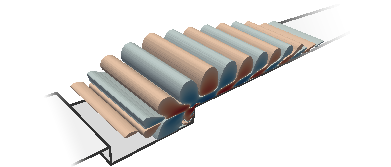
\includegraphics{Images/2D_3Dmode/pdfs/d4w19_2dmode.pdf}
		\caption{Two-dimensional mode}\label{fig:2Dmode}
	\end{subfigure}
	\begin{subfigure}{0.495\linewidth}
		\centering
		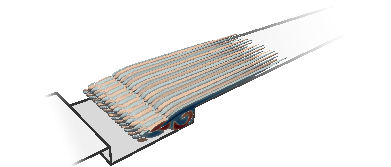
\includegraphics{Images/2D_3Dmode/pdfs/d4w19_3dmode.pdf}
		\caption{Three-dimensional mode}\label{fig:3Dmode}
	\end{subfigure}\\[10pt]
	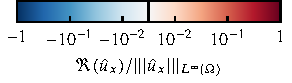
\includegraphics{Images/2D_3Dmode/pdfs/colorbar.pdf}
	\caption{Real part of the streamwise component of the most unstable (a) two-dimensional and (b) three-dimensional modes for the gap configuration $(w,d)=(19,4)$ at $\Rey=1000$. The modes are visualised using isosurfaces of $\Re(\hat{u}_x)$ on a two-sided logarithmic scale.}\label{fig:modes}
\end{figure}

The two modes are localised differently. The two-dimensional mode stays close to the gap, with a comparatively uniform amplitude near its downstream edge, whereas the three-dimensional mode extends far downstream in the form of long streamwise streaks. These streaks are much weaker than the mode structure inside the cavity. The two modes are also well separated in frequency: here $\omega_{\mathrm{3D}}\approx0.0256$, which is about an order of magnitude below $\omega_{\mathrm{2D}}\approx0.2457$, so the three-dimensional structures evolve on a much slower time scale than the shear-layer oscillation. A frequency separation of comparable magnitude between the three-dimensional mode and the two-dimensional shear-layer mode is also reported for open cavities \citep{bresColonius2008}.

Both modes can be identified with the two families reported for compressible gaps by \citet{mathiasMedeiros2019,mathiasMedeiros2021} and \citet{aguirreMedeiros2024}. The two-dimensional mode is an oscillation of the shear layer spanning the gap and corresponds to their Rossiter modes. In compressible flow, the Rossiter feedback loop is closed by acoustic waves propagating upstream from the downstream edge \citep{rossiter1964}. In the incompressible limit the pressure responds instantaneously to the impingement of the shear layer on that edge, so the feedback becomes purely hydrodynamic but the shear-layer oscillation persists. The three-dimensional mode, concentrated in the recirculating region inside the cavity, corresponds to their centrifugal modes. It arises from a centrifugal instability of the closed streamlines of the recirculating vortex. This mechanism has already been identified in incompressible open cavities by \citet{meseguerGarrido2014}, \citet{deVicente2014} and \citet{Citro2015}, and shown by \citet{bresColonius2008} to depend only weakly on the Mach number (for $M<0.6$). The same physical mechanisms therefore appear to underlie both the present incompressible modes and the compressible modes of Medeiros and co-workers. One difference is that the partition of \citet{aguirreMedeiros2024} contains no region in which only the two-dimensional mode is unstable, whereas such a region (III and IV) is found here for wide, shallow gaps.

\section{Two-dimensional dynamics}\label{sec:2Ddynamics}
Building on the correspondence between the two-dimensional stability boundary and the experimental transition boundary, the nonlinear two-dimensional dynamics of flow over gapped surfaces are examined. A systematic nonlinear \ac{DNS} parameter sweep is performed over gap depths $d$, gap widths $w$, and Reynolds numbers $\Rey$. The two-dimensional dynamical regimes identified at $\Rey=1000$ are summarised in figure~\ref{fig:2Ddynamics1000}.

\begin{figure}[ht]
	\centering
	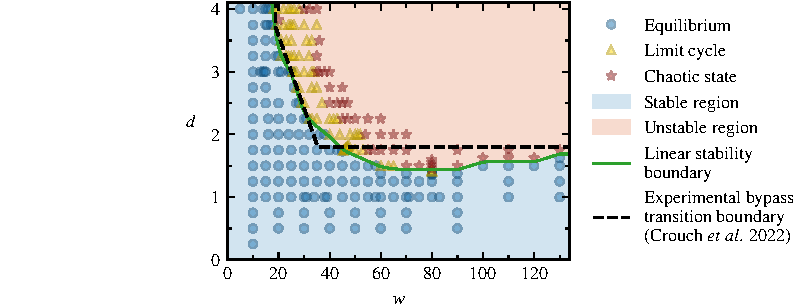
\includegraphics{Images/inc2dStabilityCurveRe1000.pdf}
	\caption{Limit set classification over the parameter space $0\leq w \leq 130$ and $0 \leq d \leq 4$ at $\Rey = 1000$. Blue circles denote equilibrium states, yellow triangles denote limit cycles, and red stars denote chaotic states. The continuous green line represents the linear stability boundary separating the locally stable and unstable regimes, shaded in blue and red respectively. The dashed black line represents the experimental boundary beyond which flow transition is observed at the gap location rather than through downstream primary instability mechanisms \citep{jeffGaps}.}\label{fig:2Ddynamics1000}
\end{figure}
As noted in Section~\ref{sec:globalStability}, for sufficiently small gap depths and widths the flow asymptotically approaches an equilibrium state. For deeper gaps, increasing the width takes the flow through a sequence of bifurcations that ends in chaotic dynamics. The first of these is a supercritical Hopf bifurcation (solid green line in figure~\ref{fig:2Ddynamics1000}), at which the equilibrium gives way to a stable periodic orbit. Widening the gap further eventually destroys the periodic orbit in favour of chaotic motion. The full route to two-dimensional chaos has not been mapped out here, because transition at the gap is a three-dimensional process (Section~\ref{sec:3Ddynamics}) and the two-dimensional chaotic states are therefore of limited physical relevance. Nevertheless, several period-doubling bifurcations have been identified along the way (Section~\ref{sec:bifurcations}), which are a classical signature of the period-doubling route to chaos.

The shape of the stability boundary in figure~\ref{fig:2Ddynamics1000} is itself informative, as the critical depth varies non-monotonically with the gap width. Moving from left to right along the boundary, the critical depth first decreases, so that progressively shallower gaps become unstable, until it reaches a minimum near $(w,d)\approx(75,1.5)$, where the two steps of the gap interact most strongly. Beyond that width the trend reverses: the critical depth increases with $w$, so that widening a gap of fixed depth becomes stabilising. For even wider gaps, the coupling between the two steps weakens and the critical depth approaches the value set by two isolated steps. Additional \ac{DNS} of isolated steps, performed in the present study at $\Rey=1000$, place the onset of global instability at $d\in(2.75,3.0]$ for the \ac{FFS} and at $d\in(3,3.25]$ for the \ac{BFS}, and show that very wide gaps ($w\gg 250$) are required to reach this asymptotic limit.

\subsection{\ac{TS} waves amplification (2D stable regime)}\label{sec:2Dstable}
\ac{TS} waves are the dominant primary convective instability mechanism in two-dimensional laminar boundary layers. However, laminar boundary layers are globally stable to two-dimensional perturbations \citep{ehrensteinGallaire2005}. Therefore, a continuous source of noise is required to excite \ac{TS} waves. To evaluate and corroborate the \ac{TS}-wave amplification trends reported experimentally by \citet{jeffGaps}, linearised simulations are performed about the equilibrium base states $\boldsymbol{U}$ obtained from \ac{DNS} (blue circles in figure~\ref{fig:2Ddynamics1000}; regions I and II in figure~\ref{fig:3d2dDynamics1000}). A body force $\boldsymbol{f}={(f_x,f_y)}^\mathrm{T}$ is added to the right-hand side of~\eqref{eq:linearizedNS} to excite \ac{TS} waves. The forcing $\boldsymbol{f}$ has a divergence-free Gaussian spatial envelope and is multiplied by a zero-mean, unit-variance Gaussian white-noise signal $X_t$:
\begin{align}
	f_x(\boldsymbol{x},t) & = -(y-y_{\mathrm{c}}) \exp\big({-\kappa{|\boldsymbol{x}-\boldsymbol{x}_{\mathrm{c}}|}^2}\big) X_t, \\
	f_y(\boldsymbol{x},t) & = (x-x_{\mathrm{c}}) \exp\big({-\kappa{|\boldsymbol{x}-\boldsymbol{x}_{\mathrm{c}}|}^2}\big) X_t,
\end{align}
where $\kappa = 100$, $\boldsymbol{x}_{\mathrm{c}} ={(x_{\mathrm{c}},y_{\mathrm{c}})}^\mathrm{T} = {(-95, 0.5)}^\mathrm{T}$ and $|\cdot|$ denotes the Euclidean norm. The spatial envelope confines the forcing to a small circular region centred at $\boldsymbol{x}_{\mathrm{c}}$. Although ambient disturbances in experiments are neither strictly white nor Gaussian noise, this stochastic model provides a standard and reproducible representation of the external forcing. The sensitivity of the results to the size of the forcing region and to the power spectrum of the input signal is assessed in Appendix~\ref{app:forcing}.

The linearised system is integrated forward in time until the initial transient has decayed and a statistically stationary response is reached. The amplification is then quantified in two steps: first a streamwise-dependent scalar disturbance amplitude $A(x)$ is extracted from the solution, and then that amplitude is converted into an $n$-factor.

The amplitude at a streamwise position $x$ is taken to be the wall-normal $L^2$ norm of the velocity perturbation,
\begin{equation}
	A(x) := {\||\boldsymbol{u}'|\|}_{L^2(\mathcal{Y}(x))} = {\left( \int_{\mathcal{Y}(x)} ({u_x'}^2 + {u_y'}^2) \mathrm{d}y\right)}^{1/2},
	\label{eq:amplitudeNorm}
\end{equation}
where $\mathcal{Y}(x)$ denotes the wall-normal section at $x$. Because the forcing is stochastic, the response fluctuates in time, and~\eqref{eq:amplitudeNorm} is replaced by
\begin{equation}
	A(x) := {\left( \int_{\mathcal{Y}(x)} {\langle {u_x'}^2 + {u_y'}^2\rangle}_\mathcal{T}\, \mathrm{d}y\right)}^{1/2},
	\label{eq:amplitudeTimeAverage}
\end{equation}
where ${\langle \cdot \rangle}_\mathcal{T}$ denotes temporal expectation over the stationary stochastic ensemble defined in the time interval $\mathcal{T}$.

Following the classical $e^n$ method \citep{smithgamberoni,vanIngen1956}, the growth of this amplitude relative to a reference position $x_0$ is measured by the local $n$-factor,
\begin{equation}
	n_{x_0}(x) = \log\left(\frac{A(x)}{A(x_0)} \right).
\end{equation}
The reference position $x_0$ is taken to be the location of minimum disturbance amplitude upstream of the gap. For brevity, the subscript is omitted hereafter, $n\equiv n_{x_0}$.

The amplification measured in this way can be compared with the prediction of local stability theory which, unlike the global stability results, resolves the contribution of each individual frequency. Local \ac{LSA} is therefore performed on the same equilibrium base flows at discrete streamwise positions, excluding the immediate vicinity of the gap corners, where the parallel-flow approximation is not valid. Because the forcing is white in time, the boundary layer is excited over a band $\mathcal{F}$ of real frequencies. Thus, the spatial formulation of the Orr--Sommerfeld problem is the relevant one: at each position $x$ the wall-normal section $U(y;x)$ of the base flow is considered and~\eqref{eq:OS} is solved for a prescribed real frequency $\omega_\mathrm{r}\in\mathcal{F}$. The least stable mode $\alpha(x;\omega_\mathrm{r})$ and its associated eigenvector $\hat{\boldsymbol{u}}(y;x,\omega_\mathrm{r})$ are retained. The eigenvector is taken such that its $L^2$ norm over the wall-normal section $\mathcal{Y}(x)$ is one. % chktex 8

Since the base flow varies in $x$, the wavenumber does too, and the strictly parallel ansatz~\eqref{eq:localansatz} must be replaced by its slowly varying counterpart. The perturbation is then written, in the manner of a WKBJ (Wentzel--Kramers--Brillouin--Jeffreys) approximation, as the superposition
\begin{equation}
	\boldsymbol{u}'(x,y,t)
	=
	\int_{\mathcal{F}}\hat{\boldsymbol{u}}(y;x,\omega_\mathrm{r})
	\mathrm{e}^{n(x;\omega_\mathrm{r})}\exp\left(\mathrm{i}\int_{x_0}^{x}\alpha_\mathrm{r}(\xi;\omega_\mathrm{r})\mathrm{d}\xi\right)
	\mathrm{e}^{-\mathrm{i}\omega_\mathrm{r} t}\mathrm{d}\omega_\mathrm{r},
\end{equation}
where
\begin{equation}
	n(x;\omega_\mathrm{r}) := \int_{x_0}^{x} -\alpha_\mathrm{i}(\xi;\omega_\mathrm{r})\,\mathrm{d}\xi,
\end{equation}
so that $-\alpha_\mathrm{i}$ is the local spatial growth rate and $n(x;\omega_\mathrm{r})$ the $n$-factor accumulated by that frequency alone between $x_0$ and $x$. Taking $\mathcal{T}=(0,\infty)$, the time-averaged amplitude~\eqref{eq:amplitudeTimeAverage} reduces to
\begin{equation}	A^2(x) = \int_{\mathcal{F}} \mathrm{e}^{2 n(x;\omega_\mathrm{r})}\mathrm{d}\omega_\mathrm{r},
\end{equation}
which yields the local version of the $n$-factor,
\begin{equation}\label{eq:localnfactor}
	n(x) = \frac{1}{2}\log\left(\frac{1}{|\mathcal{F}|}\int_{\mathcal{F}} \mathrm{e}^{2 n(x;\omega_\mathrm{r})}\,\mathrm{d}\omega_\mathrm{r}\right),
\end{equation}
where $|\mathcal{F}|$ is the measure of the frequency band. For the configurations considered, $\mathcal{F}=[0,600]$, which is wider than the broadest unstable band of frequencies (see figure~\ref{fig:neutralcurves}), so that the integral in~\eqref{eq:localnfactor} is dominated by unstable modes.

\begin{figure}[ht]
	\centering
	\begin{subfigure}{0.497\linewidth}
		\centering
		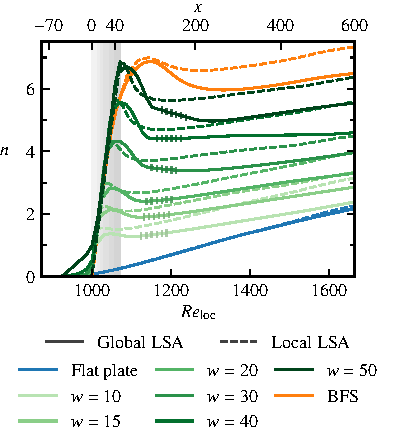
\includegraphics{Images/nfactorCurvesLocald1.5.pdf}
		\caption{Gaps with constant depth $d=1.5$.}\label{fig:nfactorCurvesA}
	\end{subfigure}
	\begin{subfigure}{0.497\linewidth}
		\centering
		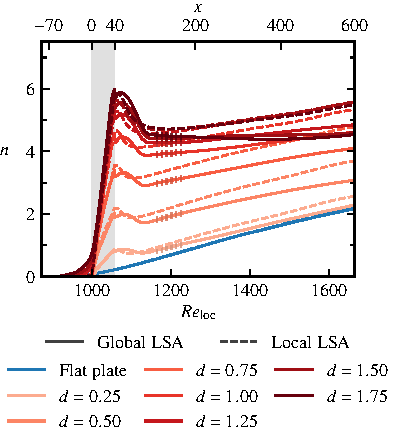
\includegraphics{Images/nfactorCurvesLocalw40.pdf}
		\caption{Gaps with constant width $w=40$.}\label{fig:nfactorCurvesB}
	\end{subfigure}
	\caption{Streamwise evolution of the $n$-factor for different gap configurations at $\Rey=1000$, from the global analysis (solid) and from the local analysis (dashed). Small markers indicate the streamwise locations used to compute the average $\Delta n$ of~\eqref{eq:deltan}. The flat-plate reference case is shown as a blue line and the \ac{BFS} case as a orange line.}\label{fig:nfactorCurves}
\end{figure}
Figure~\ref{fig:nfactorCurves} shows the streamwise evolution of the $n$-factor at $\Rey=1000$ for gaps of different widths and depths, obtained from both global and local analysis. Streamwise positions are shown through either $x$ or the local Reynolds number based on the displacement thickness of the undisturbed Blasius boundary layer at that position,
\begin{equation}\label{eq:reyLoc}
	\Rey_\mathrm{loc}(x) := u_\infty \delta_\mathrm{loc}^*(x)/\nu = \Rey\sqrt{1 + C^2 x/ \Rey},
\end{equation}
with $C\approx1.7208$. In figure~\ref{fig:nfactorCurvesA}, the gap depth is fixed at $d=1.5$ and the width is varied over $w\in[10,50]$, while in figure~\ref{fig:nfactorCurvesB}, the gap width is fixed at $w=40$ and the depth is varied over $d\in[0.25,1.75]$. In all cases, the first step of the gap starts at $x=0$, and the shaded band spans across the length of the gap. The curves show a similar overall trend. Within the gap, $n$ increases rapidly and reaches a maximum before the downstream edge. A similar peak in $n$ was also observed experimentally by \citet{jeffGaps}. Downstream of the gap, $n$ decreases significantly before recovering a monotonic growth trend similar to that of the flat-plate reference, although with some streamwise variation in slope. Global and local \ac{LSA} results agree closely. The local model reproduces the steep rise of $n$ across the gap, the maximum near the downstream edge, the drop that follows and the recovery at the flat-plate rate. The agreement is particularly good up to the peak of the $n$-factor curve. However, the local model does overestimate the amplification downstream. Downstream, far from the gap, the base flow resembles a Blasius profile, so the local growth rates, and with them the slopes of the local $n$-factor curves, become almost indistinguishable from those of the flat-plate case. The global results instead show a visibly smaller slope, and the discrepancy originates over the gap itself, where the flow is strongly non-parallel. There the low-frequency waves that the local analysis predicts to be convectively unstable downstream leave the gap having accumulated less amplification than the local model assigns them, which flattens the $n$-factor curves downstream of the gap.

For the constant-depth cases in figure~\ref{fig:nfactorCurvesA}, the \ac{BFS} case is also included for reference. The \ac{BFS} produces the largest amplification, with the gap results approaching this value as the gap width increases, in agreement with the predictions of \citet{jeffGaps}. Moreover, due to the absence of a second step, the abrupt drop observed in the gap cases is not present in the \ac{BFS} curve. Instead, a more gradual decrease and smoother $n$-factor profile is observed. The differences in the subsequent recovery of the $n$ curves after the initial drop are less clear. This is particularly evident in figure~\ref{fig:nfactorCurvesB}, where the deeper gaps $(d\geq1.25)$ recover more slowly than the shallower gaps, resulting in intersections between some of the curves. To investigate the origin of these trends, figure~\ref{fig:neutralcurves} shows the neutral local stability curves $\{\mathcal{D}(\alpha,\omega)=0:\alpha,\omega\in\mathbb{R}\}$ of~\eqref{eq:OS} using the same equilibrium base flows and gap configurations as in figure~\ref{fig:nfactorCurves}. There, frequencies are shown using the reduced frequency $F=10^6\omega_\mathrm{r}/\Rey$ \citep{schmid2001stability}, where both $\omega_\mathrm{r}$ and $\Rey$ are based on $\dstar$ at the gap rather than on the local displacement thickness. $F$ is thus proportional to the dimensional frequency and independent of the streamwise position, so that a wave of fixed physical frequency follows a horizontal line in the $(\Rey_\mathrm{loc},F)$ plane.

\begin{figure}[ht]
	\centering
	\begin{subfigure}{0.497\linewidth}
		\centering
		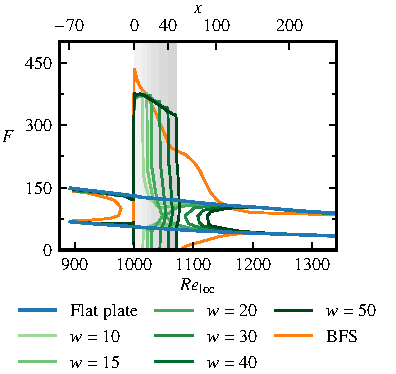
\includegraphics{Images/neutralCurvesLocald1.5.pdf}
		\caption{Gaps with constant depth $d=1.5$.}\label{fig:neutralcurvesA}
	\end{subfigure}
	\begin{subfigure}{0.497\linewidth}
		\centering
		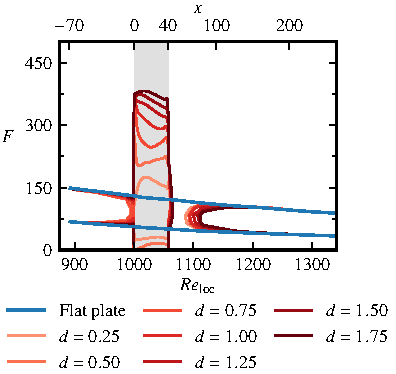
\includegraphics{Images/neutralCurvesLocalw40.pdf}
		\caption{Gaps with constant width $w=40$.}\label{fig:neutralcurvesB}
	\end{subfigure}
	\caption{Neutral curves ($\alpha_\mathrm{i}=\omega_\mathrm{i}=0$) of the Orr--Sommerfeld problem~\eqref{eq:OS}, for (a) constant gap depth $d=1.5$ with varying width $w$, and (b) constant gap width $w=40$ with varying depth $d$, compared with the flat-plate reference flow. The shaded band marks the location of the gap.}\label{fig:neutralcurves}% chktex 8
\end{figure}
Several features of the local \ac{LSA} help explain the observed behaviour of $n$ in figure~\ref{fig:nfactorCurves}. Within the cavity, the unstable frequency range broadens considerably, from the flat-plate \ac{TS} band ($55\lesssim F\lesssim130$ at $\Rey_\mathrm{loc}\approx1000$) up to $F\approx375$ for the widest and deepest gaps. Since the system is forced with white noise, all these frequencies are excited, and the strongly amplified high frequencies dominate the integral in~\eqref{eq:localnfactor}, producing the steep rise and the peak of $n$ over the gap. These high frequencies, however, are unstable only over the gap. Downstream of it they lie outside the flat-plate neutral curve and decay, so the integral is again dominated by the \ac{TS} band, which accounts for the drop of $n$ after the peak (together with the locally stable region discussed below for wider gaps). The $n$-factor therefore represents different frequencies before and after the drop, and only the latter are relevant to transition. The waves that reach a transition amplitude far downstream are those that remain unstable on the flat plate, so the level of $n$ downstream of the gap measures the additional amplification that the gap has given to the \ac{TS} frequencies, whereas the peak mostly reflects waves that do not survive beyond the gap. As a result, the height of the peak is not a measure of the effect of a gap on transition. This is clearest in figure~\ref{fig:nfactorCurvesB}: the deepest gaps produce the highest peaks, but a larger share of that growth is carried by frequencies that decay downstream, so they also undergo the largest drop and end up at levels comparable to those of shallower gaps, which gives rise to the intersections noted above.

Downstream of small gaps, such as $w=10$ and $w=15$ in figure~\ref{fig:neutralcurvesA}, the unstable region gradually approaches the flat-plate neutral boundary, so that only the \ac{TS} band remains unstable, with local growth rates close to those of the flat plate. The $n$ curves therefore recover the flat-plate slope, but not the flat-plate value. This recovery is local: the neutral curve and the local growth rate are properties of the base flow at a given position, whereas the perturbation amplitude in \ac{DNS} is the accumulated result of the entire upstream history. Two effects therefore sustain this downstream offset. First, the gap does not amplify all \ac{TS} frequencies equally. Over the gap the base flow changes rapidly in the streamwise direction, so each frequency receives a different gain on crossing it, and this gain is not given exactly by the local \ac{LSA}, which neglects these strong non-parallel effects. The \ac{TS} waves leaving the gap therefore have a different frequency content from the waves found at the same position on a flat plate, and also from that predicted by the local \ac{LSA}. Second, the problem is intrinsically advective, so this modified \ac{TS} spectrum is transported downstream and amplified multiplicatively by the local growth rates, rather than being reset by them. Consequently, even where the local stability boundaries collapse onto the flat-plate ones for $x\gg w$, the perturbation field from \ac{DNS} does not return to its flat-plate counterpart.

For wider gaps, the unstable region develops two distinct branches separated by a locally stable frequency range ($w\lesssim x\lesssim w+30$ in figure~\ref{fig:neutralcurvesB}). This locally stable region corresponds to the temporary and abrupt reduction in $n$ observed downstream of the wide gaps in figure~\ref{fig:nfactorCurves}. It also explains the slower recovery of the wider and deeper gaps shown in figure~\ref{fig:nfactorCurvesB} as the stable frequency range broadens with increasing gap width and depth.

After understanding the shape of the $n$-factor curves, the next step is to quantify the effect of a surface imperfection on transition. The metric $\Delta N$ was introduced by \citet{crouchKosoryginNg2006} and applied to gaps by \citet{jeffGaps}. This method is based on a change in the threshold value $N$ at which transition is declared, and it is constructed from the measured shift of the transition location as follows. The $n$-factor curve of the smooth reference surface, $n_\mathrm{flat}(x)$, is computed once and used throughout (the gap never enters the stability calculation). The transition location $x_\mathrm{flat}^\mathrm{trans}$ is measured in the wind tunnel for the smooth surface, giving the reference threshold $N_0=n_\mathrm{flat}(x_\mathrm{flat}^\mathrm{trans})$. For each gap configuration the transition location $x_\mathrm{gap}^\mathrm{trans}$ is then measured, and the threshold appropriate to that gap is the projected value onto the $n_\mathrm{flat}$ curve, $N=n_\mathrm{flat}(x_\mathrm{gap}^\mathrm{trans})$, so that $N=N_0-\Delta N$ with
\begin{equation}
	\Delta N := n_\mathrm{flat}\big(x_\mathrm{flat}^\mathrm{trans}\big) - n_\mathrm{flat}\big(x_\mathrm{gap}^\mathrm{trans}\big).
\end{equation}
Since a gap shifts the transition location upstream, $x_\mathrm{gap}^\mathrm{trans} < x_\mathrm{flat}^\mathrm{trans}$ and hence $\Delta N > 0$. In the present work the smooth reference is the Blasius boundary layer. The gap correlations of \citet{jeffGaps} against which the results below are compared were instead obtained for a boundary layer developing under an airfoil pressure distribution.

In the present numerical framework, the transition location cannot be determined because the governing equations are linear. A new metric $\Delta n$ is therefore used to quantify how strongly the gap amplifies the disturbances arriving from upstream. $\Delta n$ is defined as an averaged difference between the $n$-factor curve for a given gap configuration and the flat-plate reference flow, i.e.
\begin{equation}\label{eq:deltan}
	\Delta n \equiv \Delta n_\mathrm{gap}:=\frac{1}{|\mathcal{X}|}\int_{\mathcal{X}} \left(n_\mathrm{gap}(x)-n_\mathrm{flat}(x)\right)\mathrm{d}x,
\end{equation}
where $\mathcal{X}$ is a streamwise interval located downstream of the gap and $|\mathcal{X}|$ is its length. In the present study, $\mathcal{X}$ is taken to be $50$ spatial units long and to begin downstream of the initial amplitude-recovery zone, where the local growth effects of the gap and of the associated non-parallel flow have decayed. Small dashed markers on top of each amplification curve in figure~\ref{fig:nfactorCurves} represent the streamwise locations in $\mathcal{X}$ used to compute the averaged $\Delta n$ values. 

This choice of $\mathcal{X}$ captures the full amplifying effect of the gap on the band of \ac{TS} modes that are unstable at the gap location. If this band of modes is responsible for transition, the calculated $\Delta n$ can be directly linked to the transition movement. In the Blasius boundary layer, if transition is far downstream of the gap location, the band of critical modes affecting transition shifts to lower frequencies, which may be less impacted by the gap. In this case, the current $\Delta n$ would over predict the potential impacts of transition.  For applications with non-zero pressure gradients, \ac{TS}-wave growth is strongly influenced by the pressure gradient, and the shift toward lower frequencies is much less significant. In this case, the current $\Delta n$ would be more universally applicable. 

Figure~\ref{fig:nfactorsketch} illustrates qualitatively the differences between the two metrics $\Delta N$ and $\Delta n$. Comparing the two therefore requires making some assumptions. In both, $n(x)$ is the envelope of the linear modes and $N$ is the threshold value at which transition is declared. The two methods are equivalent provided that (i) transition is well correlated with a linear threshold amplitude, (ii) $\Delta n$ captures the change in linear amplitude between the gap and the reference flow, and (iii) the \ac{TS} modes that trigger transition, and thus set the measured $\Delta N$, are the ones whose amplification $\Delta n$ captures. When these three conditions hold, raising the amplification curve by $\Delta n$ and lowering the threshold by $\Delta N$ place transition at the same station, so that the two approaches yield the same result, $\Delta n=\Delta N$. 

\begin{figure}[ht]
	\centering
	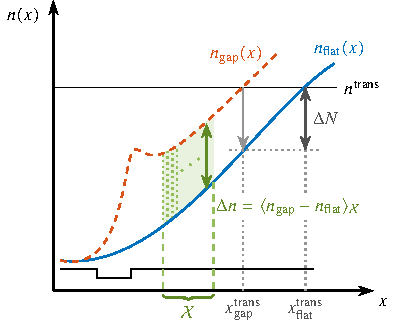
\includegraphics{Images/amplificationQualititiveNfactor.pdf}
	\caption{Schematic representation of the way the two metrics $\Delta N$ and $\Delta n$ are computed. Subscripts \textit{flat} and \textit{gap} refer to the flat-plate reference flow and the flow over a generic gap, respectively. The superscript \textit{trans} indicates the abstract transition location.}\label{fig:nfactorsketch}
\end{figure}
The metric $\Delta n$ is evaluated for all parameter configurations that admit a stable steady base flow in the two-dimensional setting. To obtain a continuous representation over the whole stable parameter domain, the computed values are interpolated using Gaussian process regression with a Matérn kernel. Figure~\ref{fig:nfactorcountour} compares the resulting numerical contours at $\Rey=1000$ (solid black lines) with the experimental isolines $\Delta N=1,2,3,4,5$ reported by \citet{jeffGaps} (dashed orange lines).

\begin{figure}[ht]
	\centering
	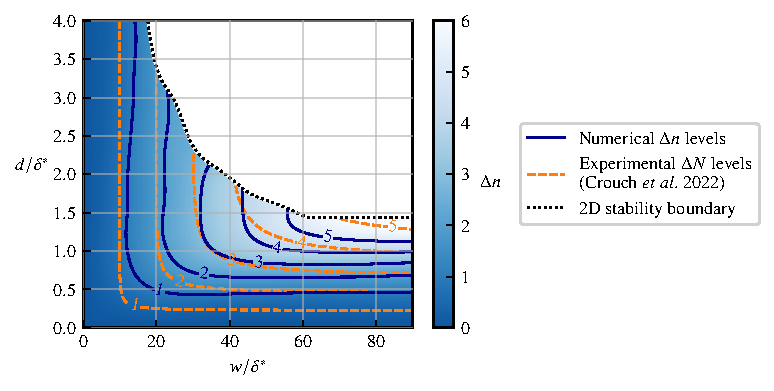
\includegraphics{Images/DeltaNcountour.pdf}
	\caption{Contour map of $\Delta n$ on the stable side of the parameter grid $(w,d)\in[0,90]\times[0,4]$ at $\Rey=1000$. Black solid contours indicate the corresponding numerical predictions. Orange dashed contours indicate experimental levels from \citet{jeffGaps} for $\Delta N=1,2,3,4, 5$. The grey region is globally unstable and is excluded.}\label{fig:nfactorcountour}
\end{figure}
The agreement between the contours of $\Delta n$ and the contours of $\Delta N$ is good. Both characteristic trends are reproduced: for narrow gaps ($w\lesssim30$), the isolines are predominantly vertical, where the amplification is primarily determined by the gap width; for shallow gaps ($d\lesssim1$), the isolines are predominantly horizontal, where the amplification is primarily determined by the gap depth. There is, however, a slight mismatch at higher $\Delta n$ values, where the numerical predictions overestimate the experimental $\Delta N$ results. There are several possible reasons for this difference.

Although the \ac{TS}-wave convective instability mechanism is two-dimensional, \citet{jeffGaps} conducted their experiments in a three-dimensional wind tunnel at low Mach number ($M<0.1$). In contrast, the present simulations use a two-dimensional domain and solve the incompressible Navier--Stokes equations. This difference in dimensionality may contribute to the observed discrepancies, while the incompressibility assumption may also play a role. The forcing model is a further source of difference. White noise excites all frequencies with equal energy, whereas in the wind tunnel free-stream turbulence, acoustic noise and surface roughness excite some frequencies more strongly than others. Since the gap amplifies each frequency by a different amount, the two measures may be dominated by different frequencies. In the simulations, $\Delta n$ is computed from the total amplitude $A(x)$, to which all forced frequencies contribute. In the experiment, $\Delta N$ is determined by the frequency that first reaches the transition threshold, and which frequency this is depends on the disturbance spectrum of the facility. Similarly, the disturbances are introduced here through a single localised source upstream of the gap, whereas in the experiment they enter the boundary layer along its whole length, including through the receptivity of free-stream disturbances at the gap edges, which the present model does not represent. For a representative gap, Appendix~\ref{app:forcing} shows that the size and shape of the forcing region leave $\Delta n$ practically unchanged, within $0.03$, when the flat plate is forced in the same way as the gap, whereas a spectrum weighted towards low frequencies, typical of free-stream turbulence, lowers $\Delta n$ by up to $0.3$, which is the direction of the discrepancy at large $\Delta n$. In addition, the choice of the averaging interval $\mathcal{X}$ in~\eqref{eq:deltan} introduces a small, but non-negligible effect on the resulting $\Delta n$ values, particularly for gaps with large amplification, due to the streamwise variation of the $n$ curves. Despite these sources of discrepancy, the computed $\Delta n$ is in good qualitative agreement with the experimental $\Delta N$.% chktex 8

Finally, the effect of Reynolds number is investigated. To study the effect of Reynolds number on the amplification of upstream disturbances, it is necessary to understand first how the global instability changes with $\Rey$. The dependence of the neutral stability curve on Reynolds number is shown in figure~\ref{fig:2DdynamicsRe} for $\Rey\in[800,3000]$. Increasing $\Rey$ shifts the two-dimensional stability boundary towards smaller gap dimensions. 

\begin{figure}[ht]
	\centering
	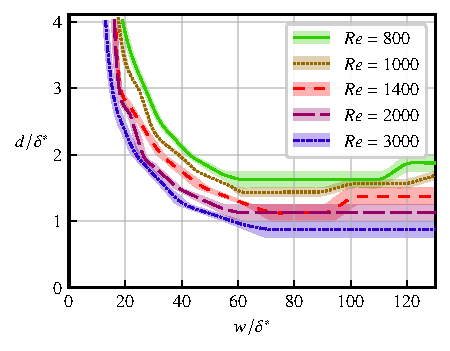
\includegraphics{Images/hopfBifReynolds.pdf}
	\caption{Global linear stability boundaries in the $(w, d)$ plane for $\Rey \in [800, 3000]$. Shaded bands indicate the uncertainty associated with interpolation between the discrete simulation points.}\label{fig:2DdynamicsRe}
\end{figure}
Figure~\ref{fig:nfactorcountourRe} shows the $\Delta n$ maps at $\Rey=800$ and $\Rey=3000$. Two effects act at the same time. First, the part of the parameter space that admits a stable steady base flow shrinks considerably as $\Rey$ increases. Second, inside the stable region the shape of the $\Delta n$ field is unchanged: the contours remain nearly vertical for narrow gaps and nearly horizontal for shallow gaps, similar to the trends observed at $\Rey=1000$.

\begin{figure}[ht]
	\centering
	\begin{subfigure}{0.497\linewidth}
		\centering
		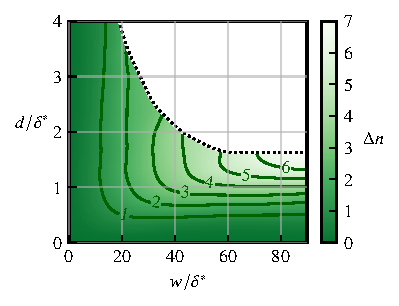
\includegraphics{Images/DeltaNcountourOnlyNumericRe800.pdf}
		\caption{$\Rey=800$}
	\end{subfigure}
	\begin{subfigure}{0.497\linewidth}
		\centering
		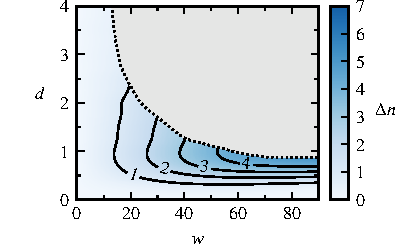
\includegraphics{Images/DeltaNcountourOnlyNumericRe3000.pdf}
		\caption{$\Rey=3000$}
	\end{subfigure}
	\caption{Contour maps of numerical predictions of $\Delta n$ over the parameter space $(w,d) \in [0,90] \times [0,4]$ for (a) $\Rey=800$ and (b) $\Rey=3000$. The dotted line is the two-dimensional stability boundary; the grey region above it is globally unstable and is excluded.}\label{fig:nfactorcountourRe}
\end{figure}
Comparing both plots in figure~\ref{fig:nfactorcountourRe} with figure~\ref{fig:nfactorcountour} shows that the two limiting regimes respond to the Reynolds number in opposite ways: for shallow gaps $\Delta n$ increases with $\Rey$, whereas for narrow gaps it decreases. The $\Delta n$ maps, however, measure only the total additional amplification supplied by a gap; they indicate neither where along the plate this amplification is acquired nor which frequencies carry it. To understand this behaviour better, and relying on the good agreement between global and local \ac{LSA}, local analysis is therefore repeated for the two opposite corners of the parameter space that remain globally stable at every Reynolds number considered: a narrow deep gap, $(w,d)=(12,4)$, and a wide shallow gap, $(w,d)=(90,0.5)$.

\begin{figure}[ht]
	\centering
	\begin{subfigure}{0.333\linewidth}
		\centering
		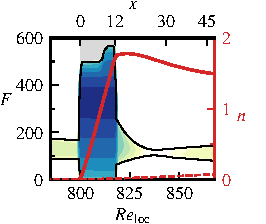
\includegraphics{Images/localMapRe800_d4_w12.pdf}
		\caption{$(w,d,\Rey)=(12,4,800)$}\label{fig:localmapsA}
	\end{subfigure}%
	\begin{subfigure}{0.333\linewidth}
		\centering
		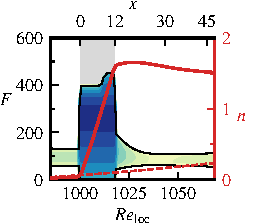
\includegraphics{Images/localMapRe1000_d4_w12.pdf}
		\caption{$(w,d,\Rey)=(12,4,1000)$}
	\end{subfigure}%
	\begin{subfigure}{0.333\linewidth}
		\centering
		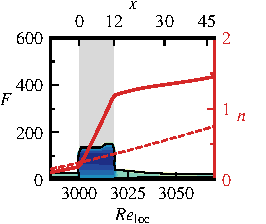
\includegraphics{Images/localMapRe3000_d4_w12.pdf}
		\caption{$(w,d,\Rey)=(12,4,3000)$}\label{fig:localmapsC}
	\end{subfigure}\\[8pt]
	\begin{subfigure}{0.333\linewidth}
		\centering
		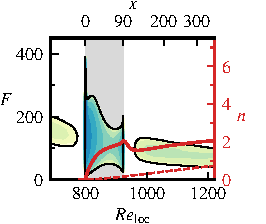
\includegraphics{Images/localMapRe800_d0.5_w90.pdf}
		\caption{$(w,d,\Rey)=(90,0.5,800)$}\label{fig:localmapsD}
	\end{subfigure}%
	\begin{subfigure}{0.333\linewidth}
		\centering
		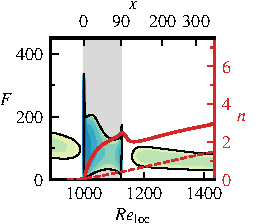
\includegraphics{Images/localMapRe1000_d0.5_w90.pdf}
		\caption{$(w,d,\Rey)=(90,0.5,1000)$}
	\end{subfigure}%
	\begin{subfigure}{0.333\linewidth}
		\centering
		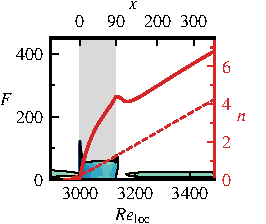
\includegraphics{Images/localMapRe3000_d0.5_w90.pdf}
		\caption{$(w,d,\Rey)=(90,0.5,3000)$}\label{fig:localmapsF}
	\end{subfigure}\\[10pt]
	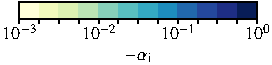
\includegraphics{Images/localMapGrowthColorbar.pdf}
	\caption{Local stability diagram and the $n$-factor it integrates to, for a narrow deep gap ($w=12$, $d=4$; top row) and a wide shallow gap ($w=90$, $d=0.5$; bottom row) at $\Rey=800$ (left column), $1000$ (middle column) and $3000$ (right column). In each panel the bottom axis is the local Reynolds number $\Rey_\mathrm{loc}$ based on the local displacement thickness of the undisturbed Blasius boundary layer \eqref{eq:reyLoc} and the top axis is the streamwise position $x$ measured from the upstream gap edge. The left axis is the reduced frequency $F=10^6\omega_\mathrm{r}/\Rey$ and the right axis the $n$-factor. The solid black line is the neutral curve $\alpha_\mathrm{i}=0$ and the filled contours inside it show the growth rate contour map. The solid red line is the $n$-factor~\eqref{eq:localnfactor} of the synthesised perturbation, and the dashed red line is its flat-plate counterpart. The shaded bands mark the location of the gaps, $0\leq x \le w$.}\label{fig:localmaps}
\end{figure}
Figure~\ref{fig:localmaps} collects, for each of the two geometries and each Reynolds number, the neutral curve $\alpha_\mathrm{i}=0$, the growth rate $-\alpha_\mathrm{i}>0$ inside it and the $n$-factor~\eqref{eq:localnfactor} that the growth rates integrate to, together with its flat-plate counterpart. The shaded band marks the gap.

In all six panels the neutral curves have qualitatively the same shape as those of figure~\ref{fig:neutralcurves}. Upstream of the gap the unstable region resembles that of the flat plate; over the gap it opens abruptly into a much broader band of frequencies, and within one or two gap widths downstream it has contracted back onto the flat-plate neutral curve. For the wide-gap case a locally stable region appears immediately upstream and downstream of the gap. Essentially all of the excess amplification is therefore produced inside the shaded band. Since $n$ is the streamwise integral of the growth rate over the amplified band, three quantities set it: the range of frequencies that band spans, the magnitude of $-\alpha_\mathrm{i}$ within it, and the distance over which it acts. Increasing $\Rey$ narrows the band but strengthens the shear layer, and which of the two prevails is decided by the width of the gap.

For the narrow deep gap (figures~\ref{fig:localmapsA}--\ref{fig:localmapsC}) the band broadens most at the lowest Reynolds number and narrows monotonically as $\Rey$ increases. The shear layer is marginally more unstable at $\Rey=3000$, but the gap is only $12$ units long, so the higher growth rates act over too short distance to offset the loss of bandwidth. The two effects do not compensate, and $\Delta n$ decreases monotonically from figure~\ref{fig:localmapsA} to figure~\ref{fig:localmapsC}. For the wide shallow gap (figures~\ref{fig:localmapsD}--\ref{fig:localmapsF}) the balance is reversed. The band is again wider at $\Rey=800$ than at $\Rey=3000$, but the growth-rate isolines at $\Rey=800$ are lower, and the gap extends over $90$ units, which is a sufficient distance for the stronger shear layer of the higher Reynolds numbers to accumulate amplification. Here $\Delta n$ increases monotonically from figure~\ref{fig:localmapsD} to figure~\ref{fig:localmapsF}. The local analysis therefore reproduces the opposite Reynolds-number trends of figure~\ref{fig:nfactorcountourRe}: narrow gaps amplify most at low $\Rey$, while wide gaps amplify most at high $\Rey$.

\subsection{Limit cycles (2D unstable regime)}\label{sec:bifurcations}
As the gap width or depth is increased the flow undergoes a supercritical Hopf bifurcation (solid green line in figure~\ref{fig:2Ddynamics1000}). The supercritical nature of the Hopf bifurcation is confirmed by the crossing of a single complex-conjugate pair of eigenvalues through the imaginary axis, while the remaining eigenvalues retain negative real parts. The expected normal-form scaling is further verified by tracking the amplitude of the emerging limit cycle along three continuation paths that cross the Hopf boundary in the $(w,d)$ plane, shown in the inset of figure~\ref{fig:hopfAmplitude}: $\boldsymbol{\gamma}_1$ crosses it by varying the gap width at fixed depth, $\boldsymbol{\gamma}_2$ along an oblique direction, and $\boldsymbol{\gamma}_3$ by varying the depth at fixed width. Defining $\epsilon:=\pm\sqrt{(w/w_\mathrm{c}-1)^2+(d/d_\mathrm{c}-1)^2}$ as the relative distance from the critical point $(w_\mathrm{c},d_\mathrm{c})$ where each path crosses the Hopf boundary, with $\epsilon>0$ on the unstable side, the real part of the critical eigenvalue is expected to increase linearly with $\epsilon$ close to the bifurcation point. The normal form for a supercritical Hopf bifurcation then predicts that the limit-cycle amplitude scales as $\sqrt{\epsilon}$, so that its square scales linearly with $\epsilon$. Figure~\ref{fig:hopfAmplitude} shows the squared $L^2$ norm of $|\boldsymbol{u}'|$ over the whole domain $\Omega$ along $\boldsymbol{\gamma}_1$ and $\boldsymbol{\gamma}_2$. In both cases it depends approximately linearly on $\epsilon$.

\begin{figure}[ht]
	\centering
	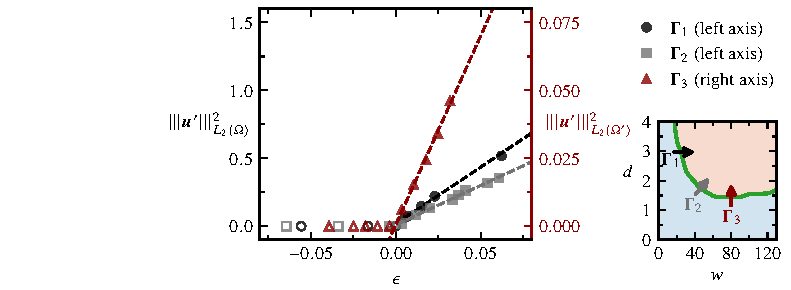
\includegraphics{Images/hopfAmplitude.pdf}
	\caption{Amplitude evolution of the limit cycle for different crossing locations of the Hopf bifurcation in the $(w, d)$ parameter plane. The three continuation paths are indicated in the small plot on the right. The abscissa $\epsilon$ is a measure of the distance from the bifurcation point along each path, so that the bifurcation lies at $\epsilon=0$ on all three paths and $\epsilon>0$ on the unstable side. Paths $\boldsymbol{\gamma}_1$ and $\boldsymbol{\gamma}_2$ (black and grey, left axis) are measured by the squared $L^2$ norm of $|\boldsymbol{u}'|$ over the whole domain $\Omega$. Path $\boldsymbol{\gamma}_3$ (dark red, right axis) is measured over $\Omega'=[w-10,w]\times[-d/2,0.5]$. Open symbols mark the stable side of the bifurcation; closed symbols mark the unstable side, and the lines are linear fits on the unstable side.}\label{fig:hopfAmplitude}
\end{figure}
The remaining path, $\boldsymbol{\gamma}_3$, crosses the Hopf boundary at fixed width $w=80$ by increasing the depth through $d\approx1.4$. A single complex-conjugate pair of eigenvalues crosses the imaginary axis here as well, yet the squared global norm does not grow linearly with $\epsilon$. This is not a failure of the normal form but a consequence of measuring the amplitude with a global norm. For gaps this wide the limit-cycle frequency has fallen to the upper edge of the band of frequencies that become convectively unstable somewhere downstream of the gap (see figure~\ref{fig:freqUnstableMode}), so the oscillation at the downstream gap edge acts as a sustained harmonic source for the boundary layer behind it. The global $L^2$ norm then mixes two contributions: the oscillation localised at the gap edge, whose amplitude does scale as $\sqrt{\epsilon}$, and the downstream wave, whose amplitude is set by the integrated convective growth rate, and hence by the domain length and by how far below the upper branch of the local neutral stability curves the frequency lies, rather than by the distance from the bifurcation point. Restricting the norm to the region $\Omega'=[w-10,w]\times[-d/2,0.5]$, which encloses the end of the shear layer up to the downstream gap edge, isolates the first contribution. Measured in $\Omega'$, the squared amplitude along $\boldsymbol{\gamma}_3$ grows linearly with $\epsilon$ close to the bifurcation (figure~\ref{fig:hopfAmplitude}), as expected from the normal form.

The fundamental frequency $\omega$ of the limit cycles varies with Reynolds number and cavity geometry, as summarised in figure~\ref{fig:freqUnstableMode}. For narrow gaps ($w\lesssim60$), the frequencies form three distinct modal branches associated with the cavity geometry and recirculation dynamics. As the gap width increases at fixed depth, the dominant mode observed for narrower gaps is replaced by a different periodic state, with a frequency characteristic of the wider cavity. The weaker interactions between branches observed across different depths indicate a secondary dependence on the gap geometry. For wide gaps ($w\gtrsim65$), the limit-cycle frequencies approach the characteristic frequency range of convectively unstable \ac{TS} waves at the corresponding Reynolds number. The associated modes have longer streamwise scales and lower frequencies.

\begin{figure}[ht]
	\centering
	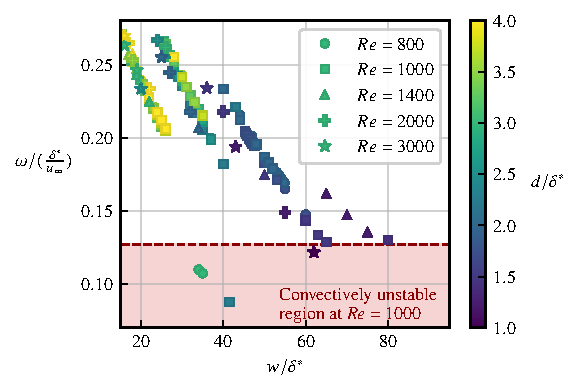
\includegraphics{Images/freqUnstableMode.pdf}
	\caption{Limit-cycle frequencies as a function of gap width $w$ for different gap depths and Reynolds numbers. Marker shading indicates gap depth, with darker markers corresponding to shallower gaps and lighter markers corresponding to deeper gaps, and marker shape denotes Reynolds number. The red shaded region indicates the approximately constant frequency range of convectively unstable \ac{TS} waves in the neighbourhood of the gap at $\Rey=1000$.}\label{fig:freqUnstableMode}
\end{figure}
Several isolated points around $w\approx40$ and $\omega\approx0.1$ in figure~\ref{fig:freqUnstableMode} correspond to states after a period-doubling bifurcation, suggesting a route from periodic to chaotic dynamics. Figure~\ref{fig:periodDoubling} illustrates one such bifurcation for two gap configurations at $\Rey=800$. Increasing the gap width from $w=33$ to $33.5$ at $d=3$ results in a limit cycle with approximately twice the period.

\begin{figure}[ht]
	\centering
	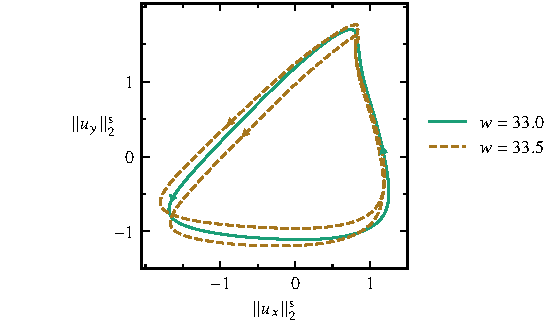
\includegraphics{Images/periodDoubling.pdf}
	\caption{Periodic orbits for the gap configurations $(w, d) = (33.0, 3)$ and $(w, d) = (33.5, 3)$ at $\Rey = 800$ projected onto the two-dimensional space $(\|u_x\|_2^\mathrm{s}, \|u_y\|_2^\mathrm{s})$. Here $\|\cdot\|_2^\mathrm{s}:=(\|\cdot\|_2-\overline{\|\cdot\|_2})/\operatorname{std}(\|\cdot\|_2)$ denotes the standardised $L^2$ norm over the computational domain, with $\operatorname{std}$ denoting the standard deviation of the corresponding time series.}\label{fig:periodDoubling}
\end{figure}
\section{Three-dimensional dynamics and transition}\label{sec:3Ddynamics}
Even though the primary convective instability of the boundary layer is two-dimensional, the global stability analysis of Section~\ref{sec:globalStability} has shown that a three-dimensional mode can become unstable before the two-dimensional one when the gap is sufficiently deep (figure~\ref{fig:3d2dDynamics1000}). This section examines the nonlinear three-dimensional dynamics in order to identify the transition scenarios that a gap can produce. Three cases are distinguished, according to which instability is active. If only the three-dimensional mode is unstable, the perturbation saturates and the downstream boundary layer remains laminar. If the equilibrium has also lost stability to two-dimensional disturbances, as happens for deep gaps, the two instabilities interact and transition is triggered at the gap itself. If instead the two-dimensional instability sets in first, as happens for wide and shallow gaps, three-dimensionality develops only further downstream. The three cases are treated in turn below.

First, region II of figure~\ref{fig:3d2dDynamics1000} is considered, where the three-dimensional mode has a positive growth rate while all two-dimensional modes are still stable. Nonlinear \ac{DNS} initialised along this mode shows the expected exponential growth, until the perturbation saturates at a finite amplitude and the flow settles onto a low-variance time-varying three-dimensional state without breaking down. Figure~\ref{fig:3dGapRegion2} shows contours of  
\begin{equation}\label{eq:3dperturbationEnergy}
	\eta:=\sqrt{{\langle|\boldsymbol{u}'|^2\rangle}_{\mathcal{Z}\times\mathcal{T}}}= {\left( \frac{1}{b}\int_{\mathcal{Z}} {\langle {u_x'}^2 + {u_y'}^2 + {u_z'}^2\rangle}_\mathcal{T}\, \mathrm{d}z\right)}^{1/2}
\end{equation}
in a neighbourhood of a gap of width $w=24$ and depth $d=2$ at $\Rey=1000$. In~\eqref{eq:3dperturbationEnergy}, $\eta$ is the square root of the spanwise- and time-averaged perturbation energy, where $\mathcal{Z}=[0,b]$ is the spanwise domain and ${\langle \cdot \rangle}_\mathcal{T}$ denotes temporal expectation over the time interval $\mathcal{T}$. This quantity is a measure of the average magnitude of the three-dimensional perturbation velocity in a spanwise 2D slice of the domain.

\begin{figure}[ht]
	\centering
	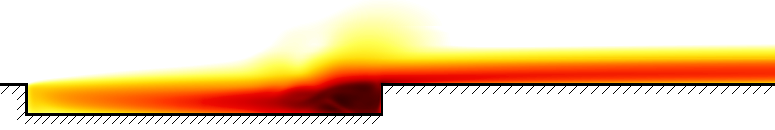
\includegraphics{Images/2dstates/pdfs/gapd2_w24_3d_originalScaling.pdf}\\[10pt]
	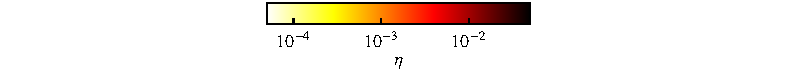
\includegraphics{Images/2dstates/pdfs/colorbar_3d.pdf}
	\caption{Distribution of the quantity $\eta$~\eqref{eq:3dperturbationEnergy} in a region surrounding the gap of dimensions $w=24$, $d=2$ at $\Rey=1000$.}\label{fig:3dGapRegion2}
\end{figure}
Figure~\ref{fig:3dGapRegion2} shows where $\eta$ resides. It is concentrated inside the cavity and around the downstream edge, where it reaches magnitudes comparable to that of the base flow, and only a weak residual extends into the rest of the gap and the boundary layer downstream of the gap, where $\eta$ is small even by comparison with the base flow. Note that this distribution is qualitatively similar to that of the three-dimensional eigenmode shown in figure~\ref{fig:3Dmode}. Downstream of the gap the three-dimensional perturbation is therefore too weak to excite the boundary layer and provoke transition on its own. However, the three-dimensional structures inside the cavity act as a sustained low-amplitude source of low-frequency noise for the boundary layer behind it, and thereby provide a continuous excitation of the \ac{TS} waves downstream. These \ac{TS} waves amplify as they are convected downstream and become visible only near the downstream boundary of the domain (not shown for brevity).

The dynamics are qualitatively different once the equilibrium becomes unstable to two-dimensional disturbances. This behaviour corresponds to region V of figure~\ref{fig:3d2dDynamics1000}.

\begin{figure}[ht]
	\centering
	\begin{subfigure}[b]{0.495\linewidth}
		\centering
		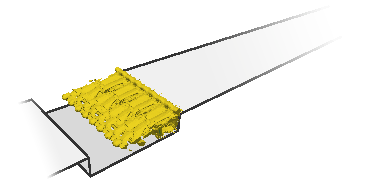
\includegraphics{Images/3DtransImages/pdfs/d4w19_3dMode_L2crit_11.pdf}
		\vspace{-1.0cm}
		\caption{$t=2310$}\label{fig:3dtransAtGap_a}
	\end{subfigure}
	\begin{subfigure}[b]{0.495\linewidth}
		\centering
		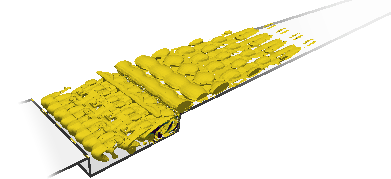
\includegraphics{Images/3DtransImages/pdfs/d4w19_3dMode_L2crit_16.pdf}
		\vspace{-1.0cm}
		\caption{$t=3710$}\label{fig:3dtransAtGap_b}
	\end{subfigure}\\
	\vspace{-0.2cm}
	\begin{subfigure}[b]{0.495\linewidth}
		\centering
		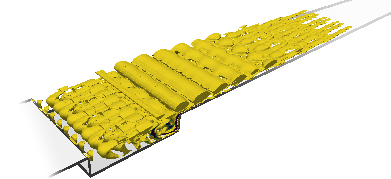
\includegraphics{Images/3DtransImages/pdfs/d4w19_3dMode_L2crit_17.pdf}
		\vspace{-1.0cm}
		\caption{$t=3990$}\label{fig:3dtransAtGap_c}
	\end{subfigure}
	\begin{subfigure}[b]{0.495\linewidth}
		\centering
		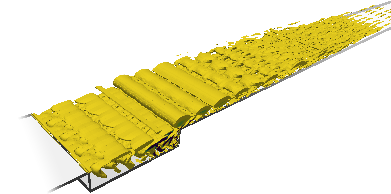
\includegraphics{Images/3DtransImages/pdfs/d4w19_3dMode_L2crit_19.pdf}
		\vspace{-1.0cm}
		\caption{$t=4550$}\label{fig:3dtransAtGap_d}
	\end{subfigure}\\
	\vspace{-0.6cm}
	\begin{subfigure}[b]{0.495\linewidth}
		\centering
		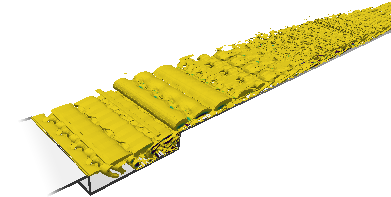
\includegraphics{Images/3DtransImages/pdfs/d4w19_3dMode_L2crit_20.pdf}
		\vspace{-1.0cm}
		\caption{$t=4830$}\label{fig:3dtransAtGap_e}
	\end{subfigure}
	\begin{subfigure}[b]{0.495\linewidth}
		\centering
		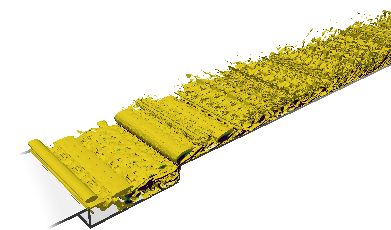
\includegraphics{Images/3DtransImages/pdfs/d4w19_3dMode_L2crit_23.pdf}
		\vspace{-1.0cm}
		\caption{$t=5670$}\label{fig:3dtransAtGap_f}
	\end{subfigure}\\
	\vspace{0.5cm}
	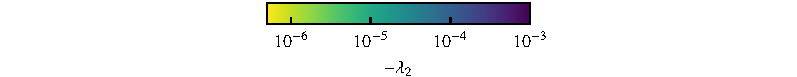
\includegraphics{Images/3DtransImages/pdfs/colorbar.pdf}
	\caption{Transition sequence for $w= 19$ and $d= 4$ at $\Rey = 1000$. Vortical structures are visualised using $\lambda_2$-criterion isosurfaces. The simulation time corresponding to each state is indicated next to each visualisation.}\label{fig:3dtransAtGap}
\end{figure}
Figure~\ref{fig:3dtransAtGap} illustrates the transition sequence for the deep-gap configuration $(w,d)=(19,4)$ at $\Rey=1000$. At this configuration the three-dimensional mode grows slightly faster than the two-dimensional one in the linear regime, so it is the first structure to emerge from a generic small disturbance. The flow initially amplifies a small perturbation along the most unstable three-dimensional eigenmode, which follows the predicted linear growth and remains confined to the cavity as a spanwise-periodic structure (figure~\ref{fig:3dtransAtGap_a}). Once nonlinear effects take over, the flow leaves the eigenmode direction and the two-dimensional mode, which is also linearly unstable, grows in turn. Two-dimensional vortices are then shed from the downstream gap edge, modulated in the spanwise direction by the three-dimensional structures in the cavity, and break up as they are advected downstream (figures~\ref{fig:3dtransAtGap_b} and~\ref{fig:3dtransAtGap_c}). The flow subsequently develops a chaotic state in the downstream boundary layer, which extends progressively towards the gap (figures~\ref{fig:3dtransAtGap_d} and~\ref{fig:3dtransAtGap_e}). At the later stages, the downstream flow exhibits increasingly complex three-dimensional structures leading to fully developed turbulence (figure~\ref{fig:3dtransAtGap_f}). Nevertheless, in the immediate vicinity of the downstream gap edge, coherent two-dimensional vortices persist and the characteristic frequency of the underlying two-dimensional oscillation remains present. This behaviour is consistent with the strong non-\ac{TS}-wave spectral peak reported experimentally by \citet{jeffGaps}.

The growth of the two-dimensional mode out of the three-dimensional one, and the subsequent breakdown, can be interpreted in terms of the triadic interactions produced by the quadratic nonlinearity of the Navier--Stokes equations, through which two Fourier components with spanwise wavenumbers and frequencies $(\beta_1,\omega_1)$ and $(\beta_2,\omega_2)$ force a third at $(\beta_1\pm\beta_2,\omega_1\pm\omega_2)$. Interacting with itself, the three-dimensional mode $(\pm\beta,\pm\omega_{\mathrm{3D}})$ forces the harmonics $(2\beta,2\omega_{\mathrm{3D}})$ and $(2\beta,0)$, and the two-dimensional components $(0,0)$ and $(0,2\omega_{\mathrm{3D}})$. The latter components correspond to a distortion of the mean flow and a slow two-dimensional oscillation, respectively. Since $2\omega_{\mathrm{3D}}\approx0.05$ is far from $\omega_{\mathrm{2D}}\approx0.25$ and also because $\omega_{\mathrm{2D}}/\omega_{\mathrm{3D}}\approx 9.6$, this self-interaction cannot force the two-dimensional mode resonantly. The two-dimensional mode is instead linearly unstable on its own at this gap configuration and grows from the small two-dimensional content already present in the flow. Conversely, once the two-dimensional oscillation $(0,\pm\omega_{\mathrm{2D}})$  is established, nonlinear interactions with the three-dimensional perturbation can generate sideband frequencies of the form $(\beta,\omega_{\mathrm{3D}}\pm k\omega_{\mathrm{2D}})$, $k\in\mathbb{N}$. The Floquet mode for the gap configuration $(w,d)=(19,4)$ at $\Rey=1000$ shown in figure~\ref{fig:3dfloquetMode} is consistent with such a modulation of the spanwise structure by the shear-layer oscillation. These interactions provide a plausible mechanism for the development of the chaotic state observed downstream of the gap, although a detailed spectral analysis would be required to confirm the associated energy transfers.

\begin{figure}[ht]
	\centering
	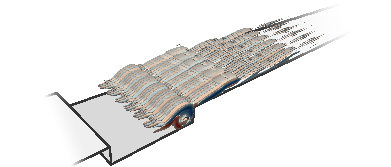
\includegraphics{Images/2D_3Dmode/pdfs/d4w19_3dFloquetmode.pdf}\\[10pt]
	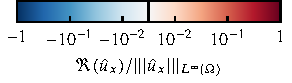
\includegraphics{Images/2D_3Dmode/pdfs/colorbar.pdf}
	\caption{Most unstable Floquet mode for the gap configuration with $w=19$ and $d=4$ at $\Rey = 1000$. The mode is visualised using isosurfaces of $\Re(\hat{u}_x)$ on a two-sided logarithmic scale.}\label{fig:3dfloquetMode}
\end{figure}
This result, together with the saturated region-II case discussed above, shows that the three-dimensional instability alone does not cause breakdown. On its own, the three-dimensional mode transfers energy only to its harmonics and to slow two-dimensional components, and it saturates. Transition at the gap requires both instabilities: the three-dimensional mode provides the spanwise structure, and the interaction of this structure with the high-frequency two-dimensional oscillation spreads energy across the spectrum and drives the flow to turbulence. 

The third scenario occupies regions III and IV of figure~\ref{fig:3d2dDynamics1000}, in which the two-dimensional instability sets in before the three-dimensional one and the resulting limit cycle remains stable to three-dimensional perturbations. The subsequent evolution of the flow is therefore governed not by a secondary three-dimensional instability, but by where the frequency of the two-dimensional oscillation falls relative to the band of convectively unstable \ac{TS} waves, which for shallow gaps lies close to the upper edge of that band (figure~\ref{fig:freqUnstableMode}). This is what distinguishes the two regions. In region III the frequency lies above the upper branch, so the oscillation is damped as it is advected downstream and the boundary layer remains laminar. In region IV the frequency lies within the band, so the oscillation is amplified downstream of the gap and transition follows through the primary pathway of \ac{TS}-wave growth.

The passage from region III to region IV is gradual, in contrast to the abrupt crossings from region I to region II or from region II to region V. Figure~\ref{fig:L2normPO} illustrates the underlying mechanism for different gap widths at fixed $d=1.5$ and $\Rey=1000$. Since the flow is now three-dimensional, the wall-normal amplitude~\eqref{eq:amplitudeNorm} is extended to include the spanwise velocity component and averaged over the spanwise period. Following the notation of~\eqref{eq:3dperturbationEnergy}, the streamwise-dependent amplitude chosen to characterise the oscillations is 
\begin{equation}\label{eq:amplitudeNorm3D}
	\|\eta\|_{L^2(\mathcal{Y}(x))} = {\left( \int_{\mathcal{Y}(x)} {\eta^2} \mathrm{d}y \right)}^{1/2} = {\left( \int_{\mathcal{Y}(x)} {\langle |\boldsymbol{u}'|^2\rangle}_{\mathcal{Z}\times\mathcal{T}}\, \mathrm{d}y \right)}^{1/2}.
\end{equation}
This quantity is shown in figure~\ref{fig:L2normPO} against distance from the downstream gap edge. The oscillation is localised at the gap edge in every case. Increasing $w$ changes the amplitude of the self-sustained oscillation near the gap and the downstream evolution of the flow. Deep within region III ($w\approx 60$) the frequency lies above the upper branch at the gap, the excited wave is damped everywhere downstream, and the norm decays to negligible values within a few hundred spatial units. As the gap widens, the structure extends farther downstream and its decay becomes progressively slower ($w\approx 63$ and $w\approx 64$). At $w=65$ the frequency lies inside the unstable band over part of the domain only. For this case, the norm grows to a maximum near $x-w\approx400$ and decays once the wave leaves that region. These four cases are computed as two-dimensional flows. For $w\gtrsim66$ the wave is amplified over the whole domain, and the two-dimensional limit cycle (dashed lines in figure~\ref{fig:L2normPOeta}) grows monotonically up to the outflow, as a train of large two-dimensional vortices.

\begin{figure}[ht]
	\centering
	\begin{subfigure}[b]{0.5\linewidth}
		\centering
		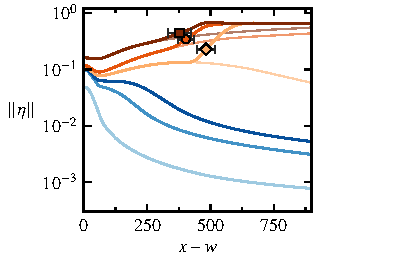
\includegraphics{Images/L2POvsX.pdf}
		\caption{Perturbation velocity}\label{fig:L2normPOeta}
	\end{subfigure}%
	\begin{subfigure}[b]{0.5\linewidth}
		\centering
		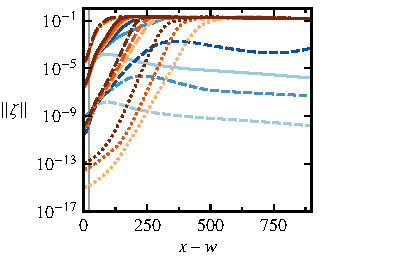
\includegraphics{Images/L2POvsXzeta.pdf}
		\caption{Spanwise perturbation velocity}\label{fig:L2normPOzeta}
	\end{subfigure}\\[6pt]
	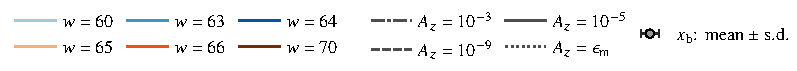
\includegraphics{Images/L2POvsXLegend.pdf}\\[10pt]
	\begin{subfigure}[b]{\linewidth}
		\centering
		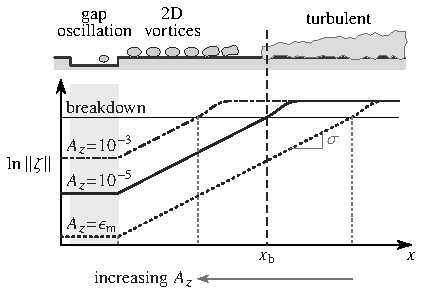
\includegraphics{Images/L2POsketch.pdf}
		\caption{Mechanism}\label{fig:L2normPOsketch}
	\end{subfigure}
	\caption{Streamwise evolution of the self-sustained oscillation for gaps of different widths at fixed depth $d=1.5$ and $\Rey=1000$. (a) Amplitude of the perturbation velocity, $\|\eta\|_{L^2(\mathcal{Y}(x))}$~\eqref{eq:amplitudeNorm3D}. The cases $w\leq65$ are two-dimensional. For $w=66$ and $w=70$, solid lines are the three-dimensional flows forced by~\eqref{eq:seedForcing} with $A=10^{-5}$, and dashed lines the two-dimensional limit cycles. The curve for $w=60$ ends at $x-w=650$, beyond which that simulation is not converged. (b) Amplitude of the spanwise perturbation velocity, $\|\zeta\|_{L^2(\mathcal{Y}(x))}$, for the three-dimensional flows with $A=10^{-5}$, $A=10^{-3}$ and without forcing ($A=0$, a single instant, $w=70$). The vertical line marks the centre of the forcing. All curves are smoothed along $x$ with a Gaussian filter of width $20$, about one \ac{TS} wavelength. (c) Sketch of the mechanism: three-dimensional disturbances grow at the rate $\sigma$ from the downstream edge of the gap, $x_0$, on the two-dimensional wave sustained by the gap, and break the flow down at $x_\mathrm{b}$, which moves upstream as their initial level increases. The flow sketch corresponds to $A=10^{-5}$.}\label{fig:L2normPO}
\end{figure}
This train of vortices is stable only in two dimensions. In three dimensions it is unstable to spanwise-varying disturbances, but the instability is convective: the disturbances grow as they are advected with the wave and leave the domain, without modifying the oscillation at the gap. The flow therefore breaks down where these disturbances have grown to a finite amplitude, and this position depends on their initial level. They are measured by the spanwise velocity, which vanishes in a two-dimensional flow, through $\|\zeta\|_{L^2(\mathcal{Y}(x))}$, defined as in~\eqref{eq:amplitudeNorm3D} with $\zeta:={\langle {u_z'}^2\rangle}_{\mathcal{Z}\times\mathcal{T}}^{1/2}$ in place of $\eta$. In the unforced simulations their level is not controlled: it is what remains of the initial perturbation once it has decayed to round-off error, so it depends on the machine precision and on how long the simulation has run. To set it explicitly, the quasi-three-dimensional simulations are restarted from their saturated state with a body force that acts only on the spanwise velocity,
\begin{equation}\label{eq:seedForcing}
	f_z = A\,E(x,y)\,Z(z)\,T(t),\qquad
	E = \mathrm{e}^{-{(x-w-20)}^2/16-{(y-1)}^2/0.5},
\end{equation}
\begin{equation}\label{eq:seedFactors}
	Z = \frac{1}{\sqrt{2}}\sum_{k=1}^{4}\cos\!\left(k\beta z+\phi_k\right),\qquad
	T = \frac{1}{\sqrt{15}}\sum_{m=1}^{30}\sin\!\left(0.01\,m\,t+\psi_m\right).
\end{equation}
Each factor is chosen so that the force seeds three-dimensional disturbances without altering the two-dimensional flow or favouring a particular disturbance. The envelope $E$ places the force inside the boundary layer, one displacement thickness from the wall and $20$ units downstream of the gap, where the two-dimensional wave has already formed; its $\mathrm{e}^{-1}$ contour is an ellipse of semi-axes $4$ and $0.7$. The spanwise factor $Z$ contains the first four harmonics of the domain, $\beta=2\pi/b$ with $b=6$, and no spanwise-uniform part, so the force does not act on the two-dimensional oscillation. The temporal factor $T$ is a multisine of $30$ lines covering $0.01\leq\omega\leq0.30$, which includes the frequency of the oscillation and its subharmonic. The phases $\phi_k$ and $\psi_m$ are random but fixed, and $Z$ and $T$ have unit root mean square, so that the amplitude $A$, the only parameter varied, is the root-mean-square force at the centre of $E$, and $A=0$ recovers the unforced simulation. Statistics are collected over $1100$--$1700$ time units, once the breakdown position no longer changes.

Figure~\ref{fig:L2normPOzeta} shows the result for $w=66$ and $w=70$. Downstream of the forcing, $\|\zeta\|_{L^2(\mathcal{Y}(x))}$ grows exponentially at the same rate, $\sigma\approx0.07$, for both widths and all forcing amplitudes, until it saturates and the flow breaks down. Taking the breakdown position $x_\mathrm{b}$ as the station where $\|\zeta\|_{L^2(\mathcal{Y}(x))}=10^{-2}$, $A=10^{-5}$ gives $x_\mathrm{b}-w\approx85$--$100$ and $A=10^{-3}$ gives $x_\mathrm{b}-w\approx30$, so that a hundredfold increase of the disturbance level moves breakdown upstream by about $\sigma^{-1}\ln100\approx65$ units. Without forcing, the only spanwise-varying content is round-off error, of order $10^{-13}$, and breakdown occurs at $x_\mathrm{b}-w\approx380$. This position is set by machine precision and is therefore not physical. It also drifted downstream as the initial perturbation decayed; had the instability been absolute, breakdown would instead have moved upstream towards the gap. For a given forcing the two widths break down at nearly the same position, although the amplitude of the two-dimensional wave there differs, $\|\eta\|_{L^2(\mathcal{Y}(x_\mathrm{b}))}\approx0.11$ for $w=66$ and $0.17$ for $w=70$. Breakdown is therefore set by the level of the three-dimensional disturbances, and not by the amplitude of the wave. Figure~\ref{fig:L2normPOsketch} summarises the mechanism: the gap oscillation sustains a two-dimensional wave, on which three-dimensional disturbances of initial level $\zeta_0$ grow convectively from the downstream edge of the gap, $x_0=w$. Breakdown then occurs at $x_\mathrm{b}-x_0\approx\sigma^{-1}\ln(\zeta_\mathrm{b}/\zeta_0)$, with $\zeta_\mathrm{b}$ the breakdown level, a distance set by the disturbance environment.


\begin{figure}[ht]
	\centering
	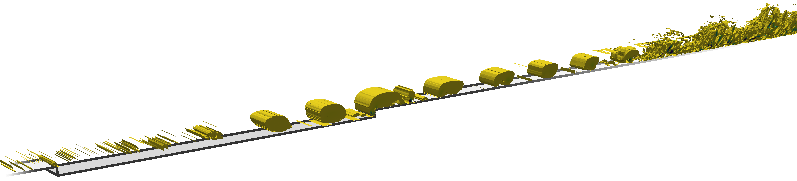
\includegraphics{Images/3DtransImages/pdfs/d1.5w80Lz5_3d_L2crit_31.pdf}\\[10pt]
	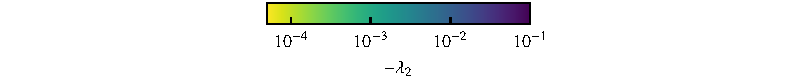
\includegraphics{Images/3DtransImages/pdfs/colorbar_w80.pdf}
	\caption{Transition scenario for a gap configuration with $w=80$ and $d=1.5$ at $\Rey = 1000$. Vortical structures are visualised using $\lambda_2$-criterion isosurfaces.}\label{fig:3dtransShallowGap}
\end{figure}
Figure~\ref{fig:3dtransShallowGap} shows this scenario for $(w,d)=(80,1.5)$, in region IV.\ Two-dimensional vortices are shed from the downstream edge of the gap and remain two-dimensional over several wavelengths, while three-dimensional disturbances grow on them, until the flow breaks down. Transition therefore takes place downstream of the gap, at a distance set by the disturbance environment. This differs from the deep-gap case of figure~\ref{fig:3dtransAtGap}, in which the two-dimensional oscillation is itself unstable to three-dimensional perturbations and the flow breaks down at the gap.

\section{Summary and discussion}\label{sec:conclusions}
We have studied how a spanwise-uniform rectangular gap affects the stability and transition of a laminar incompressible boundary layer, using \ac{DNS} and global stability analysis over the range $w\in[0,130]$, $d\in[0,4]$ and $\Rey\in[800,3000]$, which is of interest in civil aviation. We have studied the gap from two complementary viewpoints. Where the equilibrium is stable, the gap has been treated as an amplifier of incoming disturbances and characterised by the amplification increment $\Delta n$. Beyond that regime, it has been treated as a dynamical system, and the bifurcations through which it loses stability have been followed. Three results stand out.

First, the gap equilibrium loses stability through a supercritical Hopf bifurcation, and the resulting neutral curve is not monotonic in width: increasing the width, the critical depth first decreases, reaching a minimum where the two gap edges interfere most strongly, and then increases towards the isolated-step limit. Increasing the Reynolds number is destabilising and moves the whole boundary towards smaller gaps, both in width and in depth.

Second, while the equilibrium remains stable the gap acts only as an amplifier to perturbations that reach it from upstream, and this effect is fully captured by the increment $\Delta n$ obtained from stochastically forced linearised simulations. The resulting $\Delta n$ contour map shows good agreement with the $\Delta N$ experimental values measured by \citet{jeffGaps}. Local \ac{LSA} has proven opposite Reynolds-number trends followed by narrow and wide gaps. Increasing $\Rey$ narrows the band of convectively unstable frequencies but strengthens the shear layer, and the width of the gap decides which of the two prevails. In a narrow gap, the higher growth rates are confined to a short streamwise distance, so the additional amplification they provide is too small to compensate for the narrower band of unstable frequencies, and $\Delta n$ decreases as $\Rey$ increases. In a wide gap, the higher growth rates act over a long enough distance for the additional amplification to outweigh the narrower band, and $\Delta n$ increases with $\Rey$.

Third, transition at the gap is not set by the linear instability of the steady flow. The spanwise-varying mode of the equilibrium saturates and leaves the downstream boundary layer laminar; breakdown instead requires a two-dimensional limit cycle that is itself unstable to spanwise-varying perturbations. This condition is both necessary and sufficient, and the upper envelope of the spanwise-uniform and spanwise-varying neutral curves reproduces the experimental bypass boundary of \citet{jeffGaps} over the whole range considered.

These results separate two roles that a gap can play, and the distinction determines how transition should be predicted. As long as the flow over the gap remains steady, the gap merely modifies the amplification of a convective instability that it does not create; its whole effect is then contained in the single increment $\Delta n$, and the variable-$N$ method \citep{crouchKosoryginNg2006,crouch2021predicting} applies. Once the gap sustains a limit cycle that is unstable to spanwise-varying perturbations, it generates the disturbances that break the flow down itself. Transition, then, no longer proceeds through the amplification of incoming waves, and no critical $N$-factor can describe it. What separates the two regimes is a bifurcation of the flow, which can be computed directly and without calibration, and which moves towards smaller gaps as the Reynolds number increases, so that tolerances observed at one flight condition do not carry over to another.

\appendix
% jfm.cls redefines \appendix after loading hyperref, so give appendix anchors unique names
\renewcommand{\theHsection}{appendix.\Alph{section}}
\renewcommand{\theHequation}{\theHsection.\arabic{equation}}
\section{Sensitivity of \texorpdfstring{$\Delta n$}{Delta n} to the forcing}\label{app:forcing}
The increment $\Delta n$ is computed from the total amplitude~\eqref{eq:amplitudeTimeAverage}, to which every forced frequency and wavenumber contributes. It may therefore depend on how the forcing of Section~\ref{sec:2Dstable} distributes its energy, in space through the size and shape of the forcing region, and in time through the spectrum of its input signal. To quantify this dependence, the gap $(w,d)=(15,4)$ at $\Rey=1000$ is recomputed with five additional forcing cases, changing either the spatial envelope or the input signal. The averaging interval $\mathcal{T}$ and all other simulation parameters are kept constant. Each case is also applied to the flat plate, so that $n_\mathrm{gap}$ and $n_\mathrm{flat}$ in~\eqref{eq:deltan} are always computed with the same forcing. Since the equations are linear, the forcing amplitude does not affect $n$.

The envelope of Section~\ref{sec:2Dstable} is generalised to
\begin{equation}\label{eq:forcingEnvelope}
	E(\boldsymbol{x})=\exp\big(-\kappa_x{(x-x_\mathrm{c})}^2-\kappa_y{(y-y_\mathrm{c})}^2\big),
\end{equation}
which reduces to the reference Gaussian for $\kappa_x=\kappa_y=\kappa$. Its $\mathrm{e}^{-1}$ contour is an ellipse of semi-axes $\kappa_x^{-1/2}$ and $\kappa_y^{-1/2}$ (figure~\ref{fig:forcingRegions}). Four envelopes are considered: $\kappa=100$ (reference case); $\kappa=1$, of radius comparable with the displacement thickness; $\kappa=0.2$, which spans the whole boundary layer; and a strip, $(\kappa_x,\kappa_y)=(0.05,4)$, which extends along the wall over about half of a \ac{TS} wavelength and therefore filters the forced streamwise wavenumbers.

Three stationary input signals $s(t)$ are considered, each with zero mean and unit variance, ${\langle s^2\rangle}_\mathcal{T}=1$. Their power spectral density $\Phi(F)$ shows how this variance is distributed over frequency (figure~\ref{fig:forcingSpectra}). The reference signal W is discrete-time Gaussian white noise: its values at successive time steps, $\Delta t=0.006$ apart, are independent standard normal random variables. Its spectrum is therefore flat up to the Nyquist frequency $\omega_\mathrm{N}=\pi/\Delta t$ ($F_\mathrm{N}\approx5.2\times10^{5}$). However, since the frequencies amplified by the boundary layer satisfy $F\lesssim500$ even over the deepest gaps (figure~\ref{fig:neutralcurves}), most of the excited frequencies are damped immediately. The other two signals are random-phase multisines,
\begin{equation}\label{eq:multisine}
	s(t)=\sum_{k=1}^{50}a_k\sin(\omega_k t+\varphi_k),\qquad \omega_k=0.01k,
\end{equation}
which place their variance on $50$ lines covering $10\leq F\leq500$, including both the flat-plate \ac{TS} band, $55\lesssim F\lesssim130$ at $\Rey_\mathrm{loc}\approx1000$, and the higher frequencies destabilised over the gap. The amplitudes $a_k$ are equal for $\mathrm{S}_0$, giving a flat spectrum, and scale as $a_k\propto\omega_k^{-5/6}$ for $\mathrm{S}_{5/3}$, giving $\Phi\propto F^{-5/3}$. This scaling is used only as a simple low-frequency-weighted spectrum, not as a model of disturbances in a particular wind tunnel. The phases $\varphi_k$ are drawn independently and uniformly from $[0,2\pi)$, then held fixed in time. Randomising them makes the multisine ensemble stationary and prevents the sine components from adding coherently into a periodic train of pulses. The input signal multiplies both components of the force, $\boldsymbol{f}=s(t)\,{(\partial_y E,-\partial_x E)}^\mathrm{T}$, making the body force divergence-free.

\begin{figure}[ht]
	\centering
	\begin{subfigure}[b]{0.5\linewidth}
		\centering
		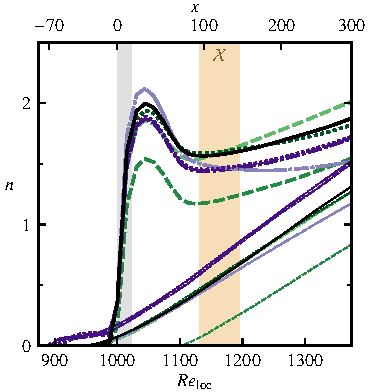
\includegraphics{Images/nfactorForcing.pdf}
		\caption{$n$-factor}\label{fig:nfactorForcing}
	\end{subfigure}%
	\begin{minipage}[b]{0.5\linewidth}
		\begin{subfigure}{\linewidth}
			\centering
			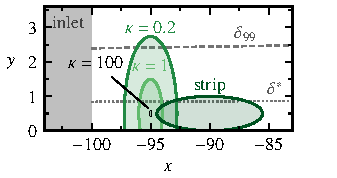
\includegraphics{Images/forcingRegions.pdf}
			\caption{Forcing envelopes}\label{fig:forcingRegions}
		\end{subfigure}\\[4pt]
		\begin{subfigure}{\linewidth}
			\centering
			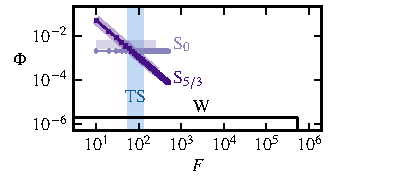
\includegraphics{Images/forcingSpectra.pdf}
			\caption{Input signals}\label{fig:forcingSpectra}
		\end{subfigure}
	\end{minipage}\\[6pt]
	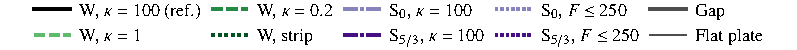
\includegraphics{Images/forcingLegend.pdf}
	\caption{Sensitivity of the $n$-factor to the forcing, for the gap $(w,d)=(15,4)$ at $\Rey=1000$. (a) $n$-factor for the eight forcings of table~\ref{tab:forcing}, for the gap (thick lines) and for the flat plate forced in the same way (thin lines). The grey band marks the gap and the orange band the interval $\mathcal{X}$ over which $\Delta n$ is averaged. (b) $\mathrm{e}^{-1}$ contours of the envelope~\eqref{eq:forcingEnvelope} for $\kappa = 0.2, 1, 100$ and for the strip $(\kappa_x,\kappa_y)=(0.05,4)$, with the boundary-layer thickness $\delta_{99}$ (dashed) and the displacement thickness $\dstar$ (dotted) of the smooth-wall boundary layer. (c) Power spectral density $\Phi$ of each input signal; for the multisines, the variance $a_k^2/2$ of each line is spread over its spacing $\Delta F=10$, $\Phi(F_k)=a_k^2/(2\Delta F)$; the wide pale bands are the multisines truncated at $F=250$. The shaded band marks the \ac{TS} frequencies unstable on the flat plate at $\Rey_\mathrm{loc}\approx1000$.}\label{fig:forcing}
\end{figure}
The resulting $n$-factor curves are shown in figure~\ref{fig:nfactorForcing}, and the corresponding values of $\Delta n$ are listed in table~\ref{tab:forcing}. In every case the gap produces the same sequence described in Section~\ref{sec:2Dstable}: rapid amplification over the gap, a peak near its downstream edge, a drop and subsequent recovery. Changing the forcing region has little effect on this sequence. Because all four envelopes use the same white-noise input, their main effect is to change the amount and type of disturbance generated by the source. A change in overall disturbance level does not change $n=\log( A(x)/A(x_0) )$, since it scales both amplitudes equally. Consistent with this, the $\kappa=1$ and strip curves nearly coincide with the reference curves over $\mathcal{X}$. The broader $\kappa=0.2$ source also excites non-\ac{TS} disturbances outside the boundary layer. These disturbances decay slowly and remain present at $x_0$, increasing the reference amplitude there and shifting both the gap and flat-plate $n$-curves down by about $0.4$. Since this shift is nearly common to both flows, it largely cancels in $\Delta n$. Thus, for the envelopes tested, the forcing region changes $\Delta n$ by no more than 3\%.

The input spectrum has a larger effect: both multisines reduce $\Delta n$, especially $\mathrm{S}_{5/3}$ (table~\ref{tab:forcing}). The measured amplitude combines the energy across the forced frequencies, so frequencies carrying more energy contribute more strongly to $n$. The gap amplifies the upper part of the flat-plate \ac{TS} band more than the lower part (figure~\ref{fig:localmaps}). Shifting input variance towards lower frequencies therefore reduces the gap's amplification relative to the flat plate. The two multisines isolate this effect because they differ only in their power spectral density. $\mathrm{S}_0$ distributes variance evenly across the forced lines, giving substantial weight to the upper \ac{TS} band and to frequencies above it. It produces the highest peak in the gap curve. By contrast, $\mathrm{S}_{5/3}$ places most of its variance below the \ac{TS} band at the gap. These lower frequencies gain less through the gap but continue to grow on the flat plate, further reducing $\Delta n$. This forcing also contains little energy at the high frequencies damped near the source, so its amplitude falls less upstream and its $n$-curves begin farther upstream. This shift is common to the gap and flat-plate cases and cancels in their difference. Truncating either multisine at $F=250$ (retaining the first $25$ lines, with the same phases and unit total variance) leaves the curves practically unchanged (table~\ref{tab:forcing}), because the removed frequencies are damped between the source at $x=-95$ and the gap.

\begin{table}
	\begin{center}
		\def~{\hphantom{0}}
		\begin{tabular}{lccccc}
			Input signal   & $\kappa_x$ & $\kappa_y$ & $x_\mathrm{c}$ & $\Delta n$ & $n-n_\mathrm{flat}$ at $x=300$ \\[3pt]
			W (reference)  & 100        & 100        & $-95$          & 1.01       & 0.56                           \\
			W              & 1          & 1          & $-95$          & 1.03       & 0.75                           \\
			W              & 0.2        & 0.2        & $-95$          & 1.04       & 0.71                           \\
			W              & 0.05       & 4          & $-90$          & 1.02       & 0.55                           \\
			$\mathrm{S}_0$          & 100        & 100        & $-95$          & 0.94       & 0.34                           \\
			$\mathrm{S}_0$, $F\leq250$ & 100     & 100        & $-95$          & 0.93       & 0.34                           \\
			$\mathrm{S}_{5/3}$      & 100        & 100        & $-95$          & 0.73       & 0.20                           \\
			$\mathrm{S}_{5/3}$, $F\leq250$ & 100 & 100        & $-95$          & 0.72       & 0.20                           \\
		\end{tabular}
		\caption{Forcings applied to the gap $(w,d)=(15,4)$ and to the flat plate at $\Rey=1000$. The table lists the input signal, envelope parameters~\eqref{eq:forcingEnvelope}, envelope centre $x_\mathrm{c}$ ($y_\mathrm{c}=0.5$ throughout), mean amplification increment $\Delta n$ over $\mathcal{X}$, and excess amplification $n_\mathrm{gap}-n_\mathrm{flat}$ at $x=300$.}\label{tab:forcing}
	\end{center}
\end{table}

Farther downstream, the forcing spectrum matters more. For every forcing, $n_\mathrm{gap}-n_\mathrm{flat}$ decreases beyond $\mathcal{X}$ because the gap curves grow more slowly than the flat-plate curves. As the unstable band shifts to lower frequencies, lower-frequency \ac{TS} waves contribute increasingly to the flat-plate amplitude; these are the frequencies amplified least by the gap. Meanwhile, the upper-frequency waves that dominate the gap response have left the unstable band and stopped growing (Section~\ref{sec:2Dstable}). The rate at which the excess decreases therefore depends on how the input variance is divided across these frequency ranges. This dependence is clearer at $x=300$: the excess is smaller for both multisines than for the white-noise reference (table~\ref{tab:forcing}). For $\mathrm{S}_0$, the gap curve is nearly flat downstream; $\mathrm{S}_{5/3}$ starts from the smallest $\Delta n$.

Over $\mathcal{X}$, changing the forcing region changes $\Delta n$ by at most $0.03$, whereas changing the spectrum changes it by up to $0.3$ (table~\ref{tab:forcing}). This spectral effect comes from how variance is distributed across frequencies, not from the upper frequency limit of the forcing: truncating at $F=250$ has negligible effect. A spectrum with more low-frequency variance would lower $\Delta n$, in the direction needed to reduce the discrepancy at large $\Delta n$ in figure~\ref{fig:nfactorcountour}, where simulations exceed measurements. These tests do not establish how much of that discrepancy is due to the experimental disturbance spectrum. Even so, both sensitivities are smaller than the spacing $\Delta N=1$ between the experimental isolines, so the comparison with the measurements of \citet{jeffGaps} is robust to the forcing choice for this gap. Farther downstream, however, the spectrum strongly affects $n$ and hence any $\Delta n$ evaluated over a later window, consistent with the dependence on the averaging interval discussed in Section~\ref{sec:2Dstable}.

\bibliographystyle{jfm}
\bibliography{jfm}

\end{document}
